\documentclass[11pt,a4paper]{article}
\usepackage[T1]{fontenc}
\usepackage{lmodern,amsmath,amssymb,bm,booktabs,tabularx,array,enumitem,xcolor,graphicx}
\usepackage[a4paper,left=24mm,right=24mm,top=23mm,bottom=23mm,headheight=14pt]{geometry}
\usepackage{fancyhdr,titlesec,tikz,listings,textcomp}
\lstset{basicstyle=\ttfamily\footnotesize,columns=fullflexible,keepspaces=true,
 breaklines=true,breakatwhitespace=false,showstringspaces=false,upquote=true,literate={Å}{{\AA}}1 {–}{{--}}1,
 aboveskip=5pt,belowskip=5pt,keywordstyle=\color{tealblue},
 commentstyle=\color{tealblue},tabsize=4}
\setcounter{tocdepth}{1}

\definecolor{tealblue}{HTML}{15585F}\definecolor{ink}{HTML}{203035}\definecolor{pale}{HTML}{EDF3F2}
\usepackage[colorlinks=true,linkcolor=tealblue,citecolor=tealblue,urlcolor=tealblue,bookmarksnumbered=true]{hyperref}
\titleformat{\section}{\Large\sffamily\bfseries\color{tealblue}}{\thesection}{.58em}{}
\titleformat{\subsection}{\large\sffamily\bfseries\color{ink}}{\thesubsection}{.55em}{}
\titlespacing*{\section}{0pt}{0pt}{8pt}\titlespacing*{\subsection}{0pt}{9pt}{3pt}
\setlength{\parindent}{0pt}\setlength{\parskip}{4.5pt plus 1pt minus 1pt}
\setlist{nosep,leftmargin=*,topsep=3pt,itemsep=2pt}\setlength{\emergencystretch}{2em}
\pagestyle{fancy}\fancyhf{}\fancyhead[L]{\small\sffamily Tensor-train kernel force fields}
\fancyhead[R]{\small\sffamily Method and implementation}
\fancyfoot[C]{\small\sffamily\thepage}\renewcommand{\headrulewidth}{0.3pt}
\newcommand{\R}{\mathbb R}\newcommand{\dd}{\mathrm d}
\newcommand{\T}{\mathsf T}\newcommand{\tr}{\operatorname{tr}}
\newcommand{\diag}{\operatorname{diag}}\newcommand{\sr}{\mathrm{sr}}
\newcommand{\phys}{\mathrm{phys}}\newcommand{\refm}{\mathrm{ref}}
\newcommand{\D}{\partial}\newcommand{\alg}[1]{\par\smallskip{\sffamily\bfseries\color{tealblue}#1}\par\nobreak}
\newcommand{\doi}[1]{\href{https://doi.org/#1}{doi:\,#1}}\newcommand{\pg}{\clearpage}
\hypersetup{pdftitle={A transferable tensor-train kernel force field},pdfauthor={P. Szabo}}
\begin{document}
\thispagestyle{plain}
{\LARGE\sffamily\bfseries\color{ink} A transferable tensor-train kernel force field\par}
{\large\sffamily\color{tealblue} Gaussian kernel fusion, tensor compression, and conservative molecular forces\par}
{\normalsize P. Szab\'o \hfill Implementation edition\quad November 2026\par}
\smallskip\hrule\medskip
\textbf{Abstract.} A product of Gaussian kernels on chemical-environment features can be evaluated exactly by summing squared distances and taking one exponential per inducing environment. We derive the corresponding sparse energy, Cartesian forces and Hessian--vector products. We then compress the same whitened inducing map across chemical feature groups. An all-center block basis provides an exact target check. A second construction factors query-side Gaussian envelopes out of a polynomial tensor train, reducing its local readout to one exponential per atom. Polynomial degree, TT bond ranks and the number of representative environments control distinct errors. One- and two-site DMRG refinements can be trained on kernel values and derivatives before the final linear fit to molecular data. Switchable D3(BJ), TS and MBD handle long-range dispersion. An executable NumPy reference and numerical checks accompany the derivations. A matched-accuracy comparison on real molecules is the proposed performance test.

\section{Energy model and intended comparison}
For a finite, isolated configuration $X=(\mathbf R,\mathbf Z)$, with $N$ atoms at Cartesian positions $\mathbf R$, take
\begin{equation}
 E(X)=\sum_{i=1}^{N}\big[e^0_{Z_i}+\epsilon_{Z_i}(x_i)-\epsilon_{Z_i}(x_{\varnothing,Z_i})\big]
       +E_{\phys}(X),\qquad
 E_{\phys}=\eta E_{\rm disp}^{(m)}+\xi E_{\rm el/pol}.
 \label{eq:model}
\end{equation}
Here $x_i$ describes atoms within $r_c$ of $i$; $x_{\varnothing,s}$ is the descriptor of an isolated atom of species $s$. The subtraction anchors the local contribution at the isolated atom. The optional electrostatic/induction baseline has its own switch $\xi$. Choose one dispersion convention $m\in\{\mathrm{D3(BJ)},\mathrm{TS},\mathrm{MBD@rsSCS}\}$ or set $\eta=0$. Use constant switches during a physical trajectory. Across all terms,
\[
 F_a=-\D_a E,\qquad H_{ab}=\D_a\D_b E=-\D_bF_a,\qquad a,b=1,\ldots,3N .
\]
The first experiment uses neutral closed-shell H/C/N/O molecules and dimers, with explicit treatment of any relevant electrostatics. Charge and spin identify electronic surfaces. Extension to ions and radical channels requires representative labels and a state-aware energy model. A geometric model trained for one surface cannot distinguish states with identical nuclear inputs.

\textbf{Success criterion.} On unseen molecules, at common force and relative-energy accuracy, reduce both total time to train (including compression) and wall time per energy-and-force evaluation. Compare full Hessians or Hessian--vector products at matched accuracy when curvature is required. All models may use accelerators. These are hypotheses to test.

\textbf{Relation to existing force fields.} Mapped sparse GPs have already removed the inducing-point loop for polynomial kernels \cite{flare}, and equivariant tensor potentials already support DMRG-type optimization \cite{etn}. The proposed test combines a transferable, species-resolved kernel with a second compression of its shared features before the reference energy fit. The question is how small its derivative-accurate ranks remain as the range of chemistry expands.

\textbf{Implementation path.} Build the fused Gaussian predictor (Sec.~\ref{sec:exact}) first. Audit the same target in a tensor basis (Sec.~\ref{sec:leaves}), then try the one-envelope polynomial TT (Sec.~\ref{sec:taylor}). Section~\ref{sec:quick} shows the fitting and inference calls. Appendix~\ref{app:code} gives the full local reference program. Section~\ref{sec:checked} reports measured checks and a readout microbenchmark.
\pg\begingroup\small\setlength{\parskip}{0pt}\tableofcontents\endgroup
\pg\section{Generate the local chemical features}
Let $\mathbf u_{ij}=\mathbf R_j-\mathbf R_i$, $r=|\mathbf u_{ij}|$, and $\hat{\mathbf u}=\mathbf u_{ij}/r$. Use $0<r_{\rm on}<r_c$. For $t=(r-r_{\rm on})/(r_c-r_{\rm on})$ define
\begin{equation}
 f_c(r)=
 \begin{cases}1&r\le r_{\rm on},\\
 1-35t^4+84t^5-70t^6+20t^7&r_{\rm on}<r<r_c,\\
 0&r\ge r_c .
 \end{cases}\label{eq:cut}
\end{equation}
Its first three derivatives match the constant branches. Neighbor-list membership can change at $r_c$ while the energy, forces, and Hessian remain continuous. Use a neighbor-list skin and evaluate the exact cutoff at each call. A physical collision at $r=0$ lies outside the model domain.

\textbf{Primitive functions.} One reproducible starting basis is $u_n(r)=f_c(r)T_n(2r/r_c-1)$ for $n=0,\ldots,n_r-1$, where $T_n$ is a Chebyshev polynomial. With real orthonormal spherical harmonics $Y_{\ell m}$, evaluate
\begin{align}
 d^i_{sn}&=\sum_{j\ne i:Z_j=s}u_n(r_{ij}),&
 A^i_{sn\ell m}&=\sum_{j\ne i:Z_j=s}u_n(r_{ij})Y_{\ell m}(\hat{\mathbf u}_{ij}),\nonumber\\
 P^i_{ab\ell}&=\sum_{m=-\ell}^{\ell} A^i_{a\ell m}A^i_{b\ell m},
   & a&=(s,n),\quad a\le b,\quad 1\le\ell\le\ell_{\max}.
 \label{eq:feat}
\end{align}
$P$ is a rotational scalar by orthogonality of the harmonic rotation matrices. Summing over neighbors enforces permutation symmetry within species. It records angular correlations including self terms. These are density-projection invariants related to SOAP and ACE \cite{soap,ace,tensorred}. Three-body invariants can have degeneracies \cite{incomplete}. For persistent torsional errors, add parity-even higher-order ACE contractions and repeat the fit.

\begin{center}\small
\begin{tabularx}{\linewidth}{@{}p{26mm}Xp{32mm}@{}}\toprule
Feature block & Deterministic list for H/C/N/O, $n_r=4$, $\ell_{\max}=3$ & Blocks / scalars\\\midrule
Radial density & For each neighbor species $s$, collect $d_{sn}$ over $n$. & 4 / 16\\
Same-species angles & For each $(s,s,\ell)$, collect $P_{(s,n)(s,n')\ell}$ for $n\le n'$. & 12 / 120\\
Mixed-species angles & For each $(s,t,\ell)$, $s<t$, collect all $n,n'$ in $P_{(s,n)(t,n')\ell}$. & 18 / 288\\\midrule
Total per center & Store the central species separately as the energy-head index. & 34 / 424\\\bottomrule
\end{tabularx}
\end{center}

\alg{Algorithm 1. From coordinates to descriptor blocks}
\begin{enumerate}
\item Use the fixed ordering H, C, N, O. For each center initialize the accumulators, enumerate its neighbors once, and accumulate $d,A$ using Eq.~\eqref{eq:feat}.
\item Contract $A$ into $P$. As an initial TT order, take the four radial blocks followed by species pairs in lexicographic order, then by $\ell$ within each pair. Reorder whole blocks using training data if this lowers bond ranks.
\item Standardize each component with training-set means and positive, floored scales. Freeze these statistics, including the convention for empty environments. Hard bond assignments, discrete hybridization labels, and globally normalized molecule features would compromise smoothness or fragment additivity.
\end{enumerate}
\pg\section{Cartesian implementation of the angular features}
An independent construction of Eq.~\eqref{eq:feat} uses only distances and dot products. It is convenient for a portable reference and avoids choosing phases for spherical harmonics. Index the $n_i$ neighbors by $j$, and the flattened species/radial channels by $a=(s,n)$. Form
\[
 U_{ja}=\mathbf 1_{Z_j=s}\,u_n(r_{ij}),\qquad
 C_{jk}=\hat{\mathbf u}_{ij}\cdot\hat{\mathbf u}_{ik},\qquad
 B_\ell=\frac{2\ell+1}{4\pi}U^\T \mathcal P_\ell(C) U .
\]
Here $\mathcal P_\ell$ is the Legendre polynomial \emph{applied entrywise}. The spherical harmonic addition theorem gives $B_\ell[a,b]=P^i_{ab\ell}$ including $j=k$ terms. The radial block is $\sum_j U_{j,:}$. Set $\mathcal P_0=1,\mathcal P_1=C$ and $(\ell+1)\mathcal P_{\ell+1}=(2\ell+1)C\odot\mathcal P_\ell-\ell\mathcal P_{\ell-1}$. Retain the upper triangle including the diagonal inside a same-species radial pair. Flatten a mixed-species block with the second radial index fastest. A zero-neighbor environment returns a zero array \emph{before} standardization. The reference uses the $O(n_i^2)$ neighbor-pair matrix to simplify differentiation. For larger neighbor counts use the spherical-harmonic accumulation in Eq.~\eqref{eq:feat} with the same normalization and compare the arrays on small environments.

\textbf{Directional differentiation without finite differences.} Carry a tuple $(f,f_u,f_v,f_{uv})$. Initialize Cartesian positions to $(\mathbf R,u,v,0)$. Linear operations act on all four entries. For any bilinear contraction $c=\mathcal L(a,b)$, including matrix products and outer products,
\begin{align*}
 c_u&=\mathcal L(a_u,b)+\mathcal L(a,b_u),\\
 c_{uv}&=\mathcal L(a_{uv},b)+\mathcal L(a_u,b_v)+
          \mathcal L(a_v,b_u)+\mathcal L(a,b_{uv}).
\end{align*}
For scalar elementwise $c=f(a)$ use $c_{uv}=f''(a)a_u a_v+f'(a)a_{uv}$. A vector-Jacobian pullback gives all forces more efficiently in a production evaluator. The two-direction implementation in the appendix makes every sign and mixed derivative independently reproducible. It avoids inverse trigonometric functions even at linear geometries. At the cutoff the branch selection uses the primal distance. Matching endpoint derivatives ensure that either neighboring branch gives the same force and Hessian there.

\textbf{Radial implementation.} Generate Chebyshev values by $T_0=1,T_1=x,T_{n+1}=2xT_n-T_{n-1}$ and multiply by $f_c$ once. The local chart is singular at coincident nuclei. Reject those inputs; if near-collisions belong to the training domain, specify a smooth physical repulsive baseline and subtract its energy and derivatives like any other baseline. Validate unit conversions before choosing a cutoff in \AA. Use the same element/radial/pair ordering in the tensor builder, fitter and deployed model.
\pg\section{The exact Gaussian model}\label{sec:exact}
Fix a central species and concatenate its descriptor blocks from Eq.~\eqref{eq:feat}. Denote the \emph{raw} blocks by $t_g$, their training means by $\mu_g$, their positive component scales by $s_g$, and their length scales by $\ell_g>0$. Division by $s_g$ is componentwise. Define $y_g=(t_g-\mu_g)/(s_g\ell_g)$, $y=\operatorname{col}_g y_g\in\R^D$. Write $z_b$ for a center already in these scaled coordinates. Both members of every comparison use the same transform. For unit-amplitude Gaussian factors,
\begin{equation}
 k(y,z_b)=\prod_{g=1}^d e^{-\|y_g-z_{bg}\|^2/2}
         =e^{-Q_b/2},\qquad Q_b=\sum_{g=1}^{d}\|y_g-z_{bg}\|^2 .
 \label{eq:fuse}
\end{equation}
Each factor treats its own coordinates. Their product is one multidimensional anisotropic Gaussian in the original descriptor, exactly. Positive scalar amplitudes would multiply into one overall amplitude. Take unit amplitude here and fit the energy scale in the readout. For overlapping linear blocks $y_g=B_g x$, the effective precision is $\sum_g B_g^\T B_g$. For a nonlinear molecular descriptor the exponent is generally nonquadratic in the Cartesian positions.

\textbf{Select bandwidths before sparsification.} Initialize component scales from training-set standard deviations with a recorded floor. Inspect the distribution of $Q$ on distinct sampled pairs for each central element. If the median is hundreds, nearly every off-diagonal kernel is essentially zero. A reproducible initialization assigns positive block weights $a_g$ with $\sum_g a_g=1$ over active blocks. Set $\ell_g^2$ to the training median nonzero standardized squared distance in block $g$ divided by $2a_g$. Remove a constant block, then multiply all lengths by a common factor to achieve a target median $Q$ (e.g.\ 2). Select this target by molecular validation. Sparse species blocks may have many exactly equal entries: track their occupancy and distances in both the full and occupied subsets.

\textbf{Select whole-environment centers.} Partition training candidates by central species. Seed rare environment families if desired, then perform pivoted Cholesky with $d_j=1$. At iteration $u$ pivot on the largest unused $d_p$ and compute
\[
 L_{ju}=\big[k(y_j,y_p)-\sum_{v<u}L_{jv}L_{pv}\big]/\sqrt{d_p},
 \qquad d_j\gets\max(0,d_j-L_{ju}^2).
\]
Stop before dividing if $d_p$ is below tolerance, or after $M$ centers. Cache one kernel column per pivot. Ties use a stable structure/atom index. When candidate pools are large this avoids storing their full Gram matrix. Save selected center coordinates and their ordering.

\textbf{Define the sparse feature map.} Diagonalize $K_{bc}=k(z_b,z_c)$ after symmetrization. Keep eigenpairs $\lambda_j>\epsilon_{\rm eig}\lambda_{\max}$, giving $r_K\le M$. Use a thin whitening factor
\begin{equation}
 W=U_{\rm keep}\Lambda_{\rm keep}^{-1/2}\in\R^{M\times r_K},\quad
 h_b(y)=k(y,z_b),\quad b(y)=W^\T h(y),\quad
 k_M(y,y')=b(y)^\T b(y'). \label{eq:nys}
\end{equation}
This is the exact evaluator of the chosen \emph{sparse} model. Sparsification already approximates the parent kernel. Eigenvalue truncation and the supervised ridge penalty operate at different stages. If a numerical jitter is used, report it and use the resulting $W$ in every comparison. Never explicitly invert $K$.

\pg\section{Fit and deploy the fused Gaussian baseline}\label{sec:fusedfit}
For a local whitened readout $w$, the scalar residual energy contribution is $\epsilon_s=b(y)^\T w=h(y)^\T c$ with $c=Ww$. Form $c$ once at export. A training row for a molecular energy sums the whitened vectors over centers of the same chemical species, subtracting their isolated-atom design contributions. The analogous force and Hessian rows follow by differentiating this sum. Section~\ref{sec:fit} gives all signs, target subtractions and weights; use the same molecules and targets for the TT.

\textbf{Single geometry.} For a scaled query $y$, define $\delta_b=y-z_b$, $a_b=c_b e^{-\|\delta_b\|^2/2}$ and $J=\partial y/\partial\mathbf R$. Reuse $a_b$ throughout:
\begin{align}
 \epsilon_s&=\sum_b a_b,& g_y&=-\sum_b a_b\delta_b,\\
 H_y v_y&=\sum_b a_b\big[\delta_b(\delta_b^\T v_y)-v_y\big],&
 F_{\rm loc}&=-J^\T g_y . \label{eq:fusedh}
\end{align}
The contribution to a Cartesian HVP is $J^\T H_y(Jv)+\sum_j(g_y)_j(\nabla^2_{\mathbf R}y_j)v$. The second term captures curvature of distances and angles. Scatter the force and HVP back to the center and every neighbor. Maintain a single sum over all affected environments for the final Cartesian arrays.

\textbf{Training rows without a derivative of the eigendecomposition.} For two Cartesian directions $u,v$, let $y_u=D_u y$, $y_v=D_v y$, $y_{uv}=D_uD_v y$, and $p_b^u=\delta_b^\T y_u$. Then
\begin{equation}
 D_u h_b=-h_b p_b^u,\qquad
 D_uD_v h_b=h_b[p_b^u p_b^v-y_u^\T y_v-\delta_b^\T y_{uv}]. \label{eq:fusejet}
\end{equation}
Multiply the resulting vectors by the frozen $W^\T$ to obtain derivatives of $b$. With $u=e_a$, the second derivative is component $a$ of a feature's Cartesian HVP. The same exponential serves every gradient and second-derivative direction at that query. Cache it while working through directions or Cartesian components.

\textbf{Batched evaluation.} For a $B_q\times D$ array $Y$ of queries and $M\times D$ training centers $Z$, compute blocks of the matrix
\[
 Q_{ib}=\|Y_i\|^2+\|Z_b\|^2-2(YZ^\T)_{ib},\qquad h_{ib}=\exp(-Q_{ib}/2).
\]
Precompute center norms. Block over queries and centers to bound memory. For nearly identical large vectors, direct differences avoid cancellation; recompute these distances before forming derivatives. Clamp only roundoff-sized negative squared distances. A hard distance or coefficient threshold inserted into the runtime energy may introduce discontinuous forces or curvature. In single precision test near coincidences, underflow and force cancellation against a double-precision reference.

\textbf{What is saved.} For $34$ blocks and $M=256$, a query requires 256 exponentials in place of 8704. Both implementations still accumulate 424 componentwise squared distances per center. This is an operation count, not a predicted wall-time factor. A BLAS-based fused implementation with gradients is the proper baseline for every claimed TT speedup.

\pg\section{Kernel multiplication, DMRG and the Gaussian limit}
Three products appear in this construction \cite{gpml,clt,oseledets}. For environments sampled in the same order the product kernel's Gram matrix is the Hadamard product $K=\bigodot_g K_g$. Ordinary matrix multiplication instead sums over an intermediate sample, $(K_1K_2)_{ij}=\sum_n K_1(i,n)K_2(n,j)$. It can represent a discretized integral operator if the measure and quadrature weights are supplied. Translation invariance and a suitable homogeneous integration measure are required to interpret that operator as a convolution.

A TT multiplies small matrices $A_g(y_g)$ and sums over \emph{bond} indices,
\[
 A_1\cdots A_d=\sum_{\alpha_1\ldots\alpha_{d-1}}
 A_1[1,\alpha_1]A_2[\alpha_1,\alpha_2]\cdots A_d[\alpha_{d-1},1]
\]
for a scalar output. A rank-one bond leaves a product. A higher rank gives a sum of products with shared subexpressions. Even if each summand is a Gaussian, the sum generally has several centers and can have signed fitted coefficients. For example $e^{-(x-a)^2/(2\ell^2)}+e^{-(x+a)^2/(2\ell^2)}$ has a local minimum at zero for $a>\ell$ and cannot be one Gaussian bell. The bare kernel in Eq.~\eqref{eq:fuse} already has separation rank one across paired blocks $(y_g,z_g)$. Compression across the blocks of the \emph{whitened inducing map} or fitted sum is where additional savings can arise.

For two Gaussian factors on the \emph{same} vector, their precisions add. If the centers differ, completing the square also supplies a constant multiplier and a precision-weighted center. Convolving normalized Gaussian densities instead adds their covariance matrices. Both identities are exact; neither turns the finite bond sum into a single term.

\textbf{What the central limit theorem implies.} For a normalized continuous stationary real positive-definite kernel $k(t)$, Bochner's theorem represents $k(t)=\mathbb E e^{i\omega^\T t}$ for a symmetric spectral probability law. If this law has finite covariance $\Sigma$, then for fixed $t$,
\[
 [k(t/\sqrt n)]^n
 =\mathbb E\exp\!\left[i t^\T n^{-1/2}\sum_{j=1}^n\omega_j\right]
 \longrightarrow e^{-t^\T\Sigma t/2},
\]
where the $\omega_j$ are independent copies. For example $\cos(t/\sqrt n)^n$ tends to $e^{-t^2/2}$. In contrast, $e^{-|t|}$ raised to the $n$th power retains a cusp at zero for every finite $n$. Distinct chemical blocks evaluated at their actual coordinates implement a different construction. The CLT therefore supplies neither an evaluation algorithm for the present TT nor a finite-rank force or Hessian error bound. A Gaussian process refers to the joint distribution of function values; it can have a non-Gaussian-shaped covariance function.

\textbf{Design decision.} Use Eq.~\eqref{eq:fuse} exactly wherever the factors are bare Gaussians. The earlier option of appending a constant to a whitened block map and renormalizing it defines a different kernel. An ablation may use that alternative, but baseline and compression must then be built from its own Gram matrices. The two TT constructions below both target Eq.~\eqref{eq:nys}.

\pg\section{Represent the same inducing map in a tensor basis}\label{sec:leaves}
In the Gaussian RKHS each block-center section is a vector. Let $q_g(y_g)$ be its coordinates in a chosen orthonormal local basis, $V_g[:,b]=q_g(z_{bg})$, and $\Phi(y)=\bigotimes_g q_g(y_g)$. The finite coefficient tensor
\begin{equation}
 \mathcal B_{p_1\ldots p_d,a}=\sum_{b=1}^M W_{ba}\prod_g V_g[p_g,b],
 \quad b_{\rm basis}(y)=\mathcal B^\T\Phi(y) \label{eq:basist}
\end{equation}
approximates the \emph{original} $b(y)$. Keep $W$ from the exact Gaussian $K$. Recomputing $W$ on an approximate product silently changes the fitting metric. The following choices distinguish basis error from bond error.

\subsection{All-center span for auditing the target}
Build $G^{(g)}_{bc}=\exp(-\|z_{bg}-z_{cg}\|^2/2)$ and its positive eigensystem $U_g^{(z)}\Lambda_g^{(z)}U_g^{(z)\T}$. Write
\begin{equation}
 T_g=\Lambda_g^{(z)-1/2}U_g^{(z)\T},\qquad
 q_g(y_g)=T_g[k_g(z_{bg},y_g)]_b,\quad V_g=T_gG^{(g)}. \label{eq:featuremap}
\end{equation}
Every section at a selected center is in the spanned space. Retaining all positive directions gives $V_g[:,b]^\T q_g(y_g)=k_g(z_{bg},y_g)$ even when $y_g$ is off the inducing set. The identity follows from $G^{(g)}T_g^\T T_g$ being the orthogonal projector onto the range of $G^{(g)}$ and the cross-kernel vector belonging to that range. Thus $b_{\rm basis}(y)=b(y)$ before any TT rounding. Duplicate sections are harmless; a nonzero numerical eigencut introduces a measurable error. Audit first and mixed derivatives using the same $T_g$. This branch may require $dM$ exponentials per query. It establishes correctness, and can be slower than the fused baseline.

\subsection{Compact block landmarks}
If the all-center span is too expensive, choose a smaller subset of each block's center coordinates by pivoted Cholesky on $G^{(g)}$. Construct $T_g$ from the subset Gram and $V_g$ from its cross Gram with \emph{all} $M$ whole environments. The deployment then requires $\sum_g M_g$ local Gaussian calls per environment. This projection has a separate error even at unrestricted TT rank. An exact check on a block-center section is its squared projection residual $1-\|V_g[:,b]\|^2$. Refit the final linear head and report molecular derivative errors. The development order is all-center span, then smaller spans or the polynomial construction in the next section.

\textbf{Shapes on disk.} Per central species store $Z[M,D]$, $W[M,r_K]$, offsets for $d$ blocks, and leaf parameters. A local leaf has width $m_g$, with $V_g[m_g,M]$. $\mathcal B$ has $r_K$ outputs. Materials in Sections~\ref{sec:leaves}--\ref{sec:sweep} only use products, thin factors and contractions. Never allocate $\mathcal B$ at full size.

\pg\section{One exponential per atom in the polynomial tensor train}\label{sec:taylor}
The Gaussian identity has a further use. For one scaled block,
\[
 k_g(y,z)=e^{-\|y\|^2/2}e^{-\|z\|^2/2}e^{y^\T z},\qquad
 e^{y^\T z}=\sum_{\alpha\in\mathbb N^{p_g}}\frac{y^\alpha z^\alpha}{\alpha!}.
\]
The multi-index $\alpha$ has $p_g$ entries, $\alpha!=\prod_j\alpha_j!$, and $y^\alpha=\prod_j y_j^{\alpha_j}$. At degree $P_g$ store only $|\alpha|\le P_g$:
\begin{equation}
 m_g=\binom{p_g+P_g}{P_g},\quad
 b_\alpha(y)=y^\alpha/\sqrt{\alpha!},\quad
 q_{g,\alpha}(y)=e^{-\|y\|^2/2}b_\alpha(y). \label{eq:taylor}
\end{equation}
At a center, store both factors in $V_g$ during construction. At a query, leave the Gaussians out of every local matrix. Since the TT is multilinear in its local features, its deployed scalar readout is exactly
\begin{equation}
 \epsilon_s^{\rm TT}(y)=
 e^{-\sum_g\|y_g\|^2/2}
 \left[\prod_{g=1}^d\sum_{\alpha} U_g[:,\alpha,:]\,b_\alpha(y_g)\right]\theta_s .
 \label{eq:singleenv}
\end{equation}
Only the envelope fusion is exact at every order and rank. Replacing the infinite Gaussian expansion by a finite polynomial and truncating TT bonds are separate approximations. After export the deployed readout has \emph{one} exponential per atom, independent of the number of inducing environments and the number of descriptor blocks. Polynomial evaluation, descriptor work and contractions remain. In a width-16 block, degrees 1, 2 and 3 give 17, 153 and 969 monomials. Choose degrees separately per block and measure the cost of the whole force call.

\textbf{Generate the feature list.} Enumerate the empty index first, then nondecreasing index tuples for each total degree, in lexicographic order. A tuple stores repeated coordinate indices. If $j$ is its last index, set $b_\alpha=b_{\alpha-e_j}\,y_j/\sqrt{\alpha_j}$, starting from $b_0=1$. Precompute a parent index, coordinate index and inverse square root for each entry. This recurrence and its derivative product rules work at $y_j=0$. Every site can use a different order, including zero for a constant block. Fixed real rescalings or a common translation of data and centers preserve the RBF provided the metric and transformation are handled consistently; the polynomial projection error depends on the expansion origin.

\textbf{Screen the degree before fitting.} Writing $s=\|y\|^2$, the squared length of the omitted RKHS feature is exactly
\[
 \delta_P^2(y)=1-e^{-s}\sum_{j=0}^P s^j/j! .
\]
It is the upper-count tail probability of a Poisson variable with mean $s$ (probability of a count greater than $P$). Use a survival-function routine when the tail is small. Orthogonality gives $|k_g(y,z)-q_g(y)^\T q_g(z)|\le\delta_P(y)\delta_P(z)$. On the full tensor product the squared omitted feature norm is $1-\prod_g[1-\delta_{P_g}^2(y_g)]$. Monitor validation quantiles and stressed geometries. Large norms may make a single-origin truncation impractical. Use block landmarks or the fused Gaussian model in that regime. These value diagnostics do not bound force or curvature errors by themselves.
\pg\section{Construct the tensor train from the inducing set}\label{sec:sweep}
A TT core $U_g\in\R^{r_{g-1}\times m_g\times r_g}$, $r_0=1$, yields a matrix for each environment,
\begin{equation}
 A_g(x_g)=\sum_p U_g[:,p,:]q_{g,p}(x_g),\quad
 \psi(x)^\T=A_1(x_1)\cdots A_d(x_d),\quad
 \widehat b(x)^\T=\psi(x)^\T B . \label{eq:tt}
\end{equation}
Here $r_d$ is a retained output width and $B\in\R^{r_d\times r_K}$. An open-boundary scalar matrix product state (MPS) results by contracting the last bond with a vector. The chain is a tensor graph: its physical indices label feature groups and its bonds label retained subspaces. DMRG selects or optimizes the cores on that graph \cite{white,oseledets,als,etn}.

\begin{center}
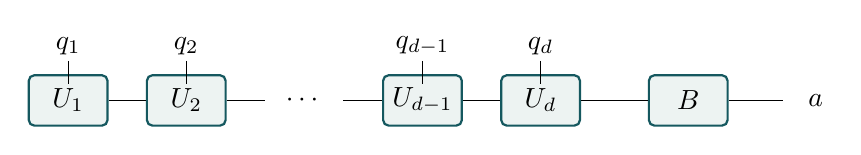
\begin{tikzpicture}[x=1.5cm,y=.67cm,core/.style={draw=tealblue,fill=pale,thick,rounded corners=2pt,minimum width=1cm,minimum height=.64cm}]
\foreach \xx/\nn in {0/1,1/2,3/{d-1},4/d}{\node[core] (u\xx) at (\xx,0) {$U_{\nn}$};\node at (\xx,1.03) {$q_{\nn}$};\draw (\xx,.75)--(\xx,.32);}
\draw (u0)--(u1);\draw (u1)--(1.67,0);\node at (2,0){$\cdots$};\draw (2.33,0)--(u3);\draw (u3)--(u4);
\node[core] (o) at (5.25,0) {$B$};\draw (u4)--(o);\draw (o)--(6.05,0);\node at (6.33,0){$a$};
\end{tikzpicture}
\end{center}

\alg{Algorithm 2. Left-to-right density-matrix truncation without a product grid}
\begin{enumerate}
\item For each $g$, store $V_g[:,b]=q_g(z_{bg})$ and $S_g=V_g^\T V_g$. Initialize $C_0$ as a row of $M$ ones. Cache suffix Hadamard products of $S_g$ (empty product is the all-ones matrix).
\item At site $g$, form the columns $J_g[:,b]=C_{g-1}[:,b]\otimes V_g[:,b]$. Trace out the unprocessed sites and the output index:
\begin{equation}
 \Gamma_g=(WW^\T)\odot\!\!\bigodot_{h>g}\! S_h,\qquad
 \rho_g=J_g\Gamma_gJ_g^\T . \label{eq:density}
\end{equation}
$\odot$ denotes entrywise multiplication. The right factors overlap through $\Gamma_g$. The retained left-prefix basis is orthonormal. Thus $\rho_g$ is the reduced Gram operator of the current unfolding of $\mathcal B$.
\item Sort its eigenvalues $\lambda_j\ge0$ in descending order. Retain the smallest $r_g$ with $\sum_{j>r_g}\lambda_j\le\delta_g^2$, subject to a rank cap. Reshape retained eigenvectors $Q_g$ into $U_g$ and set $C_g=Q_g^\T J_g$. Report any tolerance missed at the cap.
\item After site $d$, set $B=C_dW$. In the unrefined orthogonal sweep the squared Frobenius error is bounded by $\sum_g\sum_{j>r_g}\lambda_j$. For global relative tolerance $\tau$, one starting budget is $\delta_g^2=\tau^2\|\mathcal B\|_F^2/d$. This bound concerns the coefficient tensor. Derivative errors require their own tests.
\end{enumerate}
For a fixed cut, normalized eigenvalues $p_j=\lambda_j/\tr\rho_g$ also give the entropy $-\sum_jp_j\log p_j$. Compare alternative block orders using the ranks and discarded tails. A zero trace gives an empty represented subspace. For large $M$, use blocked products and apply $v\mapsto J_g[\Gamma_g(J_g^\T v)]$ in an iterative eigensolver. The direct algorithm still requires $O(M^2)$ storage per dense inducing Gram matrix.

\pg\section{Choose the DMRG sweep and the tensor graph}
\textbf{Default.} Use Algorithm 2 to initialize the shared map. Then choose \texttt{none}, \texttt{one-site}, or \texttt{two-site} refinement. Use a calibration subset of training environments. A derivative-aware target can be calculated from the uncompressed $b$, without quantum force labels:
\begin{equation}
 \mathcal J=\sum_i\!\left[
 \|\Delta b_i\|^2+
  \frac{\ell_F^2}{n_v}\sum_v\|D_v\Delta b_i\|^2+
  \frac{\ell_H^4}{n_{uv}}\sum_{u,v}\|D_uD_v\Delta b_i\|^2
 \right],\quad \Delta b_i=\widehat b(x_i)-b(x_i).
 \label{eq:sob}
\end{equation}
Here $D_v=v^\T\nabla_{\mathbf R}$ acts in physical Cartesian coordinates of the environment, for dimensionless unit directions. Set an optional term's weight to zero and omit its sum if no directions are sampled. $\ell_F,\ell_H$ are length scales. Mix sampled directions with bond stretch, bend and intermolecular displacement directions. The full kernel derivatives give teacher labels only during compression. Use held-out reference energies and forces to select the final model.

\textbf{One-site update.} In mixed-canonical form place the orthogonality center at site $g$. Let $l$ and $R$ be the contractions on either side, with the output index included in $R$. For output $a$ the local feature row is
\[
 J^{(0)}_{a;\alpha p\beta}=l_\alpha q_{g,p} R_{\beta a}.
\]
Stack rows for $\widehat b_a$, $D_v\widehat b_a$ and optional $D_uD_v\widehat b_a$ by applying the product rule to this expression, including derivatives of \emph{both} environments $l,R$. Solve the small linear least-squares problem for $\mathrm{vec}(U_g)$ with all other tensors fixed. QR in a forward sweep (RQ backward) restores the canonical gauge. Optimize the output matrix $B$ by a final linear block update. Fixed bond dimensions make memory predictable.

\textbf{Two-site update.} Merge adjacent cores into $\Theta_{\alpha p q\beta}=\sum_\nu U_g[\alpha,p,\nu]U_{g+1}[\nu,q,\beta]$. Replace $q_{g,p}$ in the local row by $q_{g,p}q_{g+1,q}$ and solve for $\Theta$. Matricize it as $(\alpha p)\mid(q\beta)$, take an SVD, and discard the smallest singular values according to the tail tolerance and rank cap. In a rightward sweep put the singular values into the right core; reverse on a leftward sweep. Increase the rank only when the validation derivatives improve. The SVD truncation error is a coefficient-norm diagnostic; re-evaluate Eq.~\eqref{eq:sob} after each split. Stop on validation plateau or a sweep budget. Joint core fitting is nonconvex even though each local solve is linear.

\textbf{Graph choice.} The default MPS is a path; evaluate it as ordinary matrix products. An optional static ML-MCTDH-style tree groups correlated blocks into common branches \cite{potfit}. At node $t$ with children $l,r$, compute $y^t_\nu=\sum_{ab}T^t_{ab\nu}y^l_a y^r_b$. Fit one node or two adjacent nodes using the same local linearization and a tree sweep. The tree changes the allowed partitions; rerunning DMRG on a path alone leaves the topology unchanged. Compare chain orders and trees using validation error at equal evaluation cost. A time propagation of these basis functions is unnecessary for a stationary force field.

\pg\section{Turn the TT sweep into numerical linear algebra}\label{sec:code_sweep}
A direct eigenproblem of dimension $r_{g-1}m_g$ in Eq.~\eqref{eq:density} can be wasteful for high polynomial degrees. Thin QR gives $J_g=Q R$ with at most $M$ columns in $Q$. Diagonalize $R\Gamma_gR^\T=U\Lambda U^\T$ and set the retained left basis to $QU_{:,1:r_g}$. Online each core has axes (left bond, physical feature, right bond). Contract the physical axis first to form an $r_{g-1}\times r_g$ matrix, then multiply the accumulated row into it. A fused implementation can contract the feature and left indices without materializing all site matrices at once.

\textbf{Indices and tolerances.} With C-order reshaping, row index $(\alpha,p)$ becomes $\alpha m_g+p$. Thus $J_g[(\alpha,p),b]=C_{g-1}[\alpha,b]V_g[p,b]$. Right factors include $WW^\T$, and the last suffix product is a matrix of ones. A suffix product is an entrywise multiplication. The coefficient norm for the initial budget is
\[
 \|\mathcal B\|_F^2=\sum_{bc}(WW^\T)_{bc}\prod_g (V_g^\T V_g)_{bc}.
\]
Take eigenvalues in descending order and keep the smallest $k$ such that the tail \emph{after} $k$ satisfies the threshold. Clip roundoff-sized negative eigenvalues and diagnose substantial indefiniteness. This spectrum belongs to the chosen local basis. Keep the exact Gaussian teacher for validation to include the error made at the leaves.

\textbf{Derivative-aware two-site solve.} For local unknown $\Theta_{\alpha p q\beta}$, a calibration observation for teacher component $j$ has feature tensor
\[
 D^0_{j,\alpha p q\beta}
    = l_\alpha\,b_{g,p}\,b_{g+1,q}\,R_{\beta j}.
\]
For Eq.~\eqref{eq:singleenv}, multiply the query envelope into $l$ exactly once. Build value and directional rows by propagating four-tuples through each outer product. Flatten $(\alpha,p,q,\beta)$ into the parameter axis, leaving $j$ as an observation axis. Form paired targets from $W^\T h$ using Eq.~\eqref{eq:fusejet}. Weight rows and right-hand sides identically. For one site remove the $q$ index. A proximal term $\zeta\|\Theta-\Theta_{\rm old}\|^2$ appends rows $\sqrt{\zeta}I$ and right-hand side $\sqrt{\zeta}\Theta_{\rm old}$. This is separate from the final energy ridge penalty.

\textbf{Gauge and memory.} Before a forward sweep, QR-factor $B^\T=Q R$, set $B\gets Q^\T$, and absorb $R^\T$ into the final site. Right-canonicalize the remaining cores by QR on their transposed right unfoldings. In a forward two-site SVD put $U$ on the left and $\Sigma V^\T$ on the right. In reverse use $U\Sigma$ and $V^\T$. Refit $B$ against all teacher components after updating cores, recompute the thin factor of $BB^\T$, and rebuild isolated-atom feature constants before the energy refit. A stale constant breaks the isolated-atom energy convention. The code assembles dense rows to expose the indexing. For production implement $D\theta$ and its adjoint $D^\T z$ as contractions, accumulate in batches, and solve without storing the design or its normal matrix.
\pg\section{Teach the compressed model with energies and derivatives}\label{sec:fit}
To retain the geometry of the projected Nystr\"om kernel, factor $BB^\T=LL^\T$ with a thin positive-eigenvalue factor. Use $\phi_s(x)=L^\T\psi(x)$, constructed independently per central species. Then $\phi_s(x)^\T\phi_s(x')=\widehat b(x)^\T\widehat b(x')$ and every resulting Gram matrix is positive semidefinite. Fitting directly in $\psi$ with a Euclidean ridge prior changes this kernel. A small terminal width $r_d$ limits the number of functions per species. Tune this width separately from the internal ranks.

\textbf{What is actually fitted.} With fixed atomic offsets $e_s^0$, define a molecule-level design vector $a(X)$ by concatenating, for each $s$,
\begin{equation}
 a_s(X)=\sum_{i:Z_i=s}[\phi_s(x_i)-\phi_s(x_{\varnothing,s})],\quad
 E_{\rm model}=E_0+E_{\phys}+a(X)^\T w,\quad E_0=\sum_i e^0_{Z_i}.
\end{equation}
Fix $e_s^0$ to isolated-atom calculations in declared states, or fit the species-count columns against training energies with their gauge documented. Composition-only training data can leave elemental offsets underdetermined. No artificial atomic energy labels are needed. Weights stored for production are $\theta_s=L_s w_s$, with $\epsilon_s=\psi_s^\T\theta_s$.

\begin{center}\small
\begin{tabularx}{\linewidth}{@{}lXX@{}}\toprule
Observation & Row acting on $w$ & Residual target\\\midrule
Energy & $a(X)^\T$ & $E_{\refm}-E_0-E_{\phys}$\\
Cartesian force $F_j$ & $-(\D_j a)^\T$ & $F^{\refm}_j-F^{\phys}_j$\\
Hessian element $H_{jk}$ & $(\D_j\D_k a)^\T$ & $H^{\refm}_{jk}-H^{\phys}_{jk}$\\
Hessian--vector component $(Hv)_j$ & $(\D_jD_v a)^\T$ & $[(H^{\refm}-H^{\phys})v]_j$\\\bottomrule
\end{tabularx}
\end{center}
If the dataset stores gradients, convert $F^{\refm}=-\nabla E^{\refm}$ once. Use consistent length/energy units for stored gradients and Hessians (energy per length and per length squared). For design matrix $A$, targets $y$ and diagonal weights $D$, solve
\begin{equation}
 \min_w\ \|D(Aw-y)\|_2^2+\lambda\|w\|_2^2. \label{eq:ridge}
\end{equation}
Example weights give a configuration a fixed total influence within each type: divide energy rows by $\sigma_E$, force rows by $\sigma_F\sqrt{3N}$, and $n_H$ selected curvature rows by $\sigma_H\sqrt{n_H}$. Choose energy residuals per molecule or per atom explicitly and apply the same scaling to the row and target. Fit conformer-energy differences using the corresponding difference of two design rows if desired.

\alg{Algorithm 3. Fit and export}
\begin{enumerate}
\item Freeze baseline settings, descriptor statistics, landmarks, chain and ranks. Evaluate $E_{\phys}$ and all derivative orders appearing in the labels with the same settings used for inference.
\item Stream complete structures, differentiating the summed atomic design. Implement $Aw$ and $A^\T v$ for LSQR/LSMR on the weighted, ridge-augmented system. Use QR on smaller problems. Tune $\lambda$ and ranks on a validation split by molecule.
\item Absorb $L_sw_s$ into the last core. Store the isolated-environment constant and elemental energy per head. Export the evaluator, baselines, element ordering and units. Training with forces alone leaves energy constants unresolved. Curvature labels are optional for evaluation of the analytic Hessian.
\end{enumerate}
\pg\section{Evaluate forces, Hessians and directional curvature}
For one local scalar readout set $l_g=A_1\cdots A_{g-1}$ and $r_g=A_{g+1}\cdots A_d\theta_s$, with identity end factors. For a Cartesian component $a$,
\begin{align}
 \D_a\epsilon_s&=\sum_g l_g(\D_a A_g)r_g,&
 \D_a A_g&=\sum_p U_g[:,p,:]\,\D_a q_{g,p}. \label{eq:force}
\end{align}
Compute all adjoints $\D\epsilon_s/\D q_{g,p}=l_g U_g[:,p,:]r_g$ in one backward pass, and pull them through the block maps and neighbor sums. Add $-\D_a\epsilon_s$ for each center whose environment depends on atom $a$, including the center itself. This gives a force on every atom from one scalar energy. Translating the entire environment gives zero derivative.

\textbf{Differentiate the geometry.} For a radial function $u(r)$,
\[
 \nabla_{\mathbf u}u=u'\hat{\mathbf u},\qquad
 \nabla^2_{\mathbf u}u=u''\hat{\mathbf u}\hat{\mathbf u}^\T+
 \frac{u'}{r}(I-\hat{\mathbf u}\hat{\mathbf u}^\T).
\]
The displacement Jacobian carries $+I$ for $j$ and $-I$ for $i$. Use Cartesian solid-harmonic recurrences divided by $r^\ell$ to evaluate $Y_{\ell m}$ without singular angular charts. Differentiate the radial/harmonic products and $P=A_a\cdot A_b$ by product rules. For a Gaussian block function with $d=x-t$,
\[
 \nabla_x h=-h\,d/\ell_g^2,\qquad
 \nabla_x^2h=h(dd^\T/\ell_g^4-I/\ell_g^2).
\]
Whitening and standardization are fixed linear/affine maps. For the polynomial TT, differentiate the shared Gaussian envelope in Eq.~\eqref{eq:singleenv} once per site energy. For any block component $q(x(\mathbf R))$, the chain rule contains both $J_x^\T(\nabla_x^2q)J_x$ and $\sum_k(\D_{x_k}q)\nabla_{\mathbf R}^2x_k$. These terms matter for vibrational frequencies.

\alg{Algorithm 4. One Hessian--vector product without constructing the Hessian}
Given a coordinate direction $v$, let a dot denote $D_v$. Form $\dot A_g$, and propagate $\dot l_{g+1}=\dot l_g A_g+l_g\dot A_g$, $\dot r_{g-1}=\dot A_g r_g+A_g\dot r_g$ with zero derivative at fixed end factors. Then
\begin{equation}
 (H_{\rm loc}v)_a=\sum_{i,g}\left[
 \dot l_g(\D_a A_g)r_g+l_g(\D_a\dot A_g)r_g+l_g(\D_a A_g)\dot r_g
 \right]_i . \label{eq:hvp}
\end{equation}
Evaluate by a forward directional pass through a reverse-mode energy gradient. Add $H_{\phys}v$ for each active baseline. A full Cartesian Hessian can be built column by column with $v=e_b$, or in sparse local blocks. Local terms may couple two atoms sharing a center even if their separation exceeds $r_c$; they vanish if the pair is farther than $2r_c$. Long-range terms can be dense. A full dense Hessian has $O(N^2)$ output cost.

\textbf{Derivative checks.} Sweep the finite-difference step $h$ and compare $v^\T F$ with $-[E(\mathbf R+hv)-E(\mathbf R-hv)]/(2h)$ and $Hv$ with $-[F(\mathbf R+hv)-F(\mathbf R-hv)]/(2h)$. Report the plateau before numerical roundoff. Check Hessian symmetry, zero net force and torque for an isolated system, and the three translational sum rules $H t_\alpha=0$. At stationary geometries project rigid translations and rotations before comparing mass-weighted vibrational eigenvalues (five rigid motions for a linear molecule).

\pg\section{Fused-envelope forces and Hessians in production}
Define $\mathcal P(y)=[\prod_g A_g^{\rm poly}(y_g)]\theta$ and $G(y)=e^{-\|y\|^2/2}$. For any direction $v_y$ in scaled descriptor space,
\begin{align}
 \epsilon&=G\mathcal P,\qquad \nabla_y\epsilon=G(\nabla_y\mathcal P-y\mathcal P),\nonumber\\
 H_y^\epsilon v_y&=G\{H_y^{\mathcal P}v_y-y(\nabla_y\mathcal P\cdot v_y)
 -(y\cdot v_y)\nabla_y\mathcal P+
 [(y\cdot v_y)y-v_y]\mathcal P\}. \label{eq:envhvp}
\end{align}
Evaluate $\mathcal P$, its gradient and its HVP by TT recurrences. Then use the Cartesian pullback below Eq.~\eqref{eq:fusedh}. A finite-difference comparison detects an omitted envelope term. A polynomial site can emit the monomial, its directional derivative and its Jacobian pullback. Differentiate the parent recurrence to avoid division by the descriptor value.

\alg{Energy, force and HVP call for a heterogeneous molecule}
\begin{enumerate}
\item Build or update the neighbor list. Set the scalar accumulator to $\sum_i e^0_{Z_i}$ and the Cartesian gradient and HVP accumulators to zero. Evaluate the physical baseline once for this structure.
\item For each center, generate raw invariant features and apply its central-species scaling. Use the fused Gaussian coefficients $c_s$, or the TT cores and terminal vector $\theta_s$. Subtract the precomputed scalar readout at the isolated environment.
\item For forces, reverse-accumulate through the site result and scatter contributions to every position in the descriptor. Return minus the accumulated gradient. For an HVP, propagate the given Cartesian direction through the same graph, differentiating the gradient. Add the baseline derivatives.
\item For a full Hessian, apply the HVP callback to Cartesian unit vectors and store the results as columns. Check the antisymmetric residual \emph{before} optional symmetrization. For vibrational modes diagonalize $M_{\rm nuc}^{-1/2}HM_{\rm nuc}^{-1/2}$ on a projected subspace at a stationary point. Return the unweighted $H$ for geometry optimization.
\end{enumerate}

\textbf{Costs to compare.} The fused Gaussian readout costs $O(MD)$ arithmetic and $M$ exponentials per atom. The fused-envelope TT costs $O(D+\sum_g m_g r_{g-1}r_g)$ arithmetic and one exponential per atom. Its cores cost $\sum_g m_gr_{g-1}r_g$ numbers plus the terminal vector. Block-landmark TT evaluation can instead entail $\sum_g M_g$ exponential calls, plus whitening and contractions. Production force and HVP implementations retain the leading arithmetic order at bounded coordination using reverse and forward-over-reverse derivatives. For energy and force fits the code forms the Cartesian Jacobian of each local descriptor in a single traversal. For an HVP the directional reference repeats passes over Cartesian components. Measure descriptor and dispersion time separately, then the end-to-end call.

\textbf{Reusing a fitted head.} Sparse output folding $c=Ww$ is exact. For a TT use the thin SVD $B=U\Sigma V^\T$, $L=U\Sigma$, and $\theta=Lw$. Updated cores, a new $B$ or new length scales invalidate cached readouts and isolated-environment constants. Persist dimensions and a model-format version so mismatched checkpoints fail before the first force call.
\pg\section{A reverse pass for all Cartesian forces}
The directional reference is an oracle for an efficient implementation. Here are explicit adjoints for the geometry path through the neighbor-pair formulation. For any intermediate $x$, write $\bar x=\partial E/\partial x$. Seed the scalar site energy with one. For the direct Gaussian, use $g_y$ in Eq.~\eqref{eq:fusedh}. For the polynomial train, one reverse pass first accumulates adjoints for its descriptor.

\textbf{Readout and monomials.} For $l_1=1$, $l_{g+1}=l_g A_g$ and $\mathcal P=l_{d+1}\theta$, seed the right vector with $\theta$. For $g=d,\ldots,1$, the adjoint for $b_{g,p}$ in $\mathcal P$ is $l_g U_g[:,p,:]r_g$, then update the right vector to $A_g r_g$. Multiply these adjoints by the envelope $G$. For each site run the monomial list in reverse. If child $c$ was computed as $b_c=b_p y_j/\sqrt{n}$, accumulate
\[
 \bar b_p\mathrel{+}=\bar b_c y_j/\sqrt{n},\qquad
 \bar y_j\mathrel{+}=\bar b_c b_p/\sqrt{n}.
\]
Add $-G\mathcal P\,y$ to the accumulated descriptor gradient for the envelope. Divide componentwise by the stored standard deviation and length-scale factors to get the raw invariant adjoints. Isolated-environment constants yield zero coordinate derivative.

\textbf{Angular and radial contractions.} For $B_\ell=c_\ell U^\T L_\ell U$, where $c_\ell=(2\ell+1)/(4\pi)$ and $L_\ell=\mathcal P_\ell(C)$, scatter the used scalar feature adjoints into an initially zero matrix $G_\ell=\bar B_\ell$. Insert each independent $(a,b)$ once; the formulas below already account for both appearances of $U$. Using the Frobenius inner product,
\begin{align*}
 \bar U&\mathrel{+}=c_\ell\,[L_\ell U G_\ell^\T+L_\ell^\T U G_\ell],\\
 \bar L_\ell&=c_\ell U G_\ell U^\T,\qquad
 \bar C\mathrel{+}=\bar L_\ell\odot\mathcal P'_\ell(C).
\end{align*}
Also distribute the radial feature adjoints to every row of $U$ through the neighbor sum. Evaluate $\mathcal P_\ell'$ by differentiating the forward Legendre recurrence, including at $C=\pm1$. For directions stored rowwise in $D$ with $C=DD^\T$, $\bar D=(\bar C+\bar C^\T)D$. For neighbor $j$, the displacement $\mathbf u$ obtains gradient
\[
 g_j=\hat{\mathbf u}\sum_n \bar U_{j,(Z_j,n)} u'_n(r)+
         (I-\hat{\mathbf u}\hat{\mathbf u}^\T)\bar D_{j,:}^\T/r .
\]
Accumulate $+g_j$ on neighbor $j$ and $-g_j$ on center $i$ in the \emph{energy gradient}. Negating once at return produces the force. The same neighbor can contribute through other centers and species heads.

\textbf{HVP at force-call complexity.} Carry $(x,\dot x)$ for direction $v$ through \emph{both} forward and reverse recurrences above. In particular $\dot{\hat{\mathbf u}}=(I-\hat{\mathbf u}\hat{\mathbf u}^\T)\dot{\mathbf u}/r$. The directional derivative of the returned energy gradient is $Hv$; differentiating forces instead gives $-Hv$. The appendix reproduces the same result by directional contractions along each Cartesian unit vector. Compare both paths and their adjoint inner products before replacing that reference with fused CPU/GPU kernels.
\pg\section{Dispersion backends I. Pairwise models}
Use atomic units inside the physical backends, recording conversions at the energy, force, and Hessian interfaces. Damping partitions short- and long-distance physics; refit residual labels for the selected convention. Each backend returns one scalar and derivatives of that same scalar.

\subsection{Grimme D3 with Becke--Johnson damping}
For a specified functional and tabulated D3(BJ) damping parameters \cite{d3,d3bj},
\begin{equation}
 E_{\rm D3(BJ)}^{(2)}=-\sum_{i<j}\sum_{n=6,8}
 \frac{s_n C_{n,ij}}{r_{ij}^{\,n}+(a_1R^0_{ij}+a_2)^n},\qquad
 R^0_{ij}=\sqrt{C_{8,ij}/C_{6,ij}}. \label{eq:d3}
\end{equation}
Compute continuous coordination numbers and interpolate element-pair reference data as defined by the D3 implementation. An isolated pair still has nonzero dispersion outside the local TT cutoff. Differentiate the geometry dependence of $C_{n,ij}$ and $R^0_{ij}$ along with the distance. Fix the optional Axilrod--Teller--Muto (ATM) three-body setting in the model specification. Include its energy and derivatives in both label subtraction and evaluation if enabled. Use the backend's tabulated data, interpolation and triplet damping consistently. Record its version, parameter record, cutoffs, and numerical accuracy. Verify smooth behavior of \emph{any} internal cutoff by scanning it. A hard far cutoff suppresses the physical tail.

For a strict smooth-separation mode, distinguish the coordination range from the dispersion range. The standard D3 coordination counting function has a small nonzero limit at infinity \cite{cncut}. Give this count a finite, smooth outer taper, e.g. Eq.~\eqref{eq:cut} at a separately specified large coordination radius. Retain the algebraic dispersion cross terms. This taper is a declared modification when the reference uses a hard coordination cutoff: use identical settings for residualization and deployment, and quantify the deviation from the original correction.

\subsection{Tkatchenko--Scheffler pair dispersion}
With volume ratio $\nu_i=V_i^{\rm eff}/V_{Z_i}^{\rm free}$, the neutral-reference TS model uses \cite{ts}
\begin{gather}
 \alpha_i=\nu_i\alpha_i^0,\qquad C_{6,ii}=\nu_i^2C_{6,ii}^0,\qquad
 R_i^{\rm vdW}=\nu_i^{1/3}R_i^0,\nonumber\\
 C_{6,ij}=\frac{2C_{6,ii}C_{6,jj}}
 {(\alpha_j/\alpha_i)C_{6,ii}+(\alpha_i/\alpha_j)C_{6,jj}},\qquad
 E_{\rm TS}=-\sum_{i<j}f_{ij}\frac{C_{6,ij}}{r_{ij}^6},\nonumber\\
 f_{ij}=\big[1+\exp\{-d_{\rm TS}(r_{ij}/[s_R(R_i^{\rm vdW}+R_j^{\rm vdW})]-1)\}\big]^{-1}.
 \label{eq:ts}
\end{gather}
Here $\alpha_i^0,C_{6,ii}^0,R_i^0$ are free-atom data for $Z_i$. Standard Hirshfeld volume ratios can be generated from reference densities with weights $h_i(\mathbf r)=\rho_i^0(\mathbf r)/\sum_j\rho_j^0(\mathbf r)$ and $\nu_i=\int |\mathbf r-\mathbf R_i|^3 h_i(\mathbf r)\rho(\mathbf r)\dd\mathbf r\big/\int |\mathbf r-\mathbf R_i|^3\rho_i^0(\mathbf r)\dd\mathbf r$. Specify the atomic reference densities and the partition convention.

\textbf{Geometry-only evaluation.} Train a separate per-species readout on $\log\nu_i$ with explicit volume labels. Set $\nu_i=\exp[g_s(x_i)-g_s(x_{\varnothing,s})]$ to anchor an isolated neutral atom at unity. Sharing the local TT features makes this inexpensive. Report volume errors separately, especially for unusual charge environments. Freeze the volume model \emph{before} producing any residual force labels, and use its predicted volumes in both fitting and deployment. Otherwise the physical contribution seen by the fit can differ from the deployed one. Learned dispersion inputs have precedents in molecular interaction models \cite{ipml,mbdml}. D3 can be implemented first when no density-derived labels are available.

\pg\section{Dispersion backend II. Many-body dispersion}\label{sec:mbd}
For finite molecules, MBD@rsSCS describes screened, coupled quantum harmonic oscillators \cite{mbd,rsscs,libmbd}. Start from positive atom-in-molecule polarizabilities and characteristic frequencies, obtained from the chosen free-atom and volume convention. For a single-pole response in atomic units,
\[
 \alpha_i(iu)=\frac{\alpha_i(0)}{1+(u/\omega_i)^2},\qquad
 \omega_i=\frac{4C_{6,ii}}{3\alpha_i(0)^2}.
\]
With the dipole-interaction sign convention in which the oscillator potential contains $+T$, construct the short-range screened response at quadrature points $u$,
\[
 \mathcal A^{\rm SCS}(iu)=\big[\mathcal A_0(iu)^{-1}+T^{\rm SR}(iu)\big]^{-1},\qquad
 \bar\alpha_i(iu)=\tfrac13\sum_j\tr_{\rm Cart}\mathcal A^{\rm SCS}_{ij}(iu).
\]
$\mathcal A_0$ is block diagonal with isotropic $3\times3$ blocks. Use the published rsSCS Gaussian-width, range-separation and Fermi-damping prescriptions with the chosen $\beta$; $T^{\rm SR}$ and the long-range interaction entering the oscillator Hamiltonian are distinct tensors. Compute $\bar C_{6,ii}=3\int_0^\infty\bar\alpha_i(iu)^2\dd u/\pi$ and $\bar\omega_i=4\bar C_{6,ii}/[3\bar\alpha_i(0)^2]$. With $\bar\alpha_i=\bar\alpha_i(0)$,
\begin{align}
 \mathcal C_{i\mu,j\nu}
 &=\delta_{ij}\delta_{\mu\nu}\bar\omega_i^2+
 (1-\delta_{ij})\bar\omega_i\bar\omega_j
 \sqrt{\bar\alpha_i\bar\alpha_j}\,T^{\rm LR}_{i\mu,j\nu},\nonumber\\
 E_{\rm MBD}&=\tfrac12\tr\sqrt{\mathcal C}-\tfrac32\sum_i\bar\omega_i .
 \label{eq:mbd}
\end{align}
Use a validated backend such as \texttt{libMBD} for quadrature, screening and finite-molecule boundary conditions. MBD includes the pair contribution through its coupling expansion. Choose it as the dispersion energy instead of summing it with TS or D3. Dense diagonalization scales as $O(N^3)$ and can dominate an inexpensive TT evaluator.

\subsection{Conservative derivatives through screening and volumes}
For $\mathcal C$ positive definite, set $S=\sqrt{\mathcal C}$. Then, for any direction $v$,
\[
 D_vE_{\rm MBD}=\tfrac14\tr(S^{-1}D_v\mathcal C)-\tfrac32\sum_iD_v\bar\omega_i,
 \qquad S\dot S+\dot S S=D_v\mathcal C .
\]
Differentiate $S^{-1}$ as $D_vS^{-1}=-S^{-1}\dot S S^{-1}$ to form mixed second derivatives, including $\D_a D_v\mathcal C$ and $\D_aD_v\bar\omega_i$. This trace formulation remains defined at equal positive eigenvalues. Monitor the smallest eigenvalue and reject or diagnose unphysical oscillators; ad hoc eigenvalue clipping can break derivative continuity.

If a backend supplies partial derivatives at fixed volumes, augment them. With $u_i=\log\nu_i$, for any backend energy $G(\mathbf R,u(\mathbf R))$,
\[
 \nabla E=G_R+J_u^\T G_u,\quad
 H=G_{RR}+G_{Ru}J_u+J_u^\T G_{uR}+J_u^\T G_{uu}J_u+
             \sum_i G_{u_i}H_{u_i}.
\]
This also applies to TS. If second partials are unavailable, compute a documented numerical HVP from centered differences of the \emph{total} analytic forces with both volumes and screening recomputed at each displaced geometry. Check step convergence. A backend claiming fixed-volume Hessians alone cannot supply the relaxed geometry-only Hessian.

\pg\section{Switch semantics and smooth separation to infinity}
\textbf{Two different uses of the switch.} Fit the local term to residual energies, forces and optional curvature for a specified physical backend and its parameters. With this same local fit, choosing $\eta=0$ removes the explicit dispersion everywhere, including inside each fragment. This is a well-defined ablation. To develop the best independent dispersion-off fit or swap D3 for MBD at fixed reference labels, recompute the residuals and refit the linear head; revalidate the basis. A finite-cutoff local fit cannot recover an omitted algebraic tail. For a common dispersion-free target, equivalent recombination requires physically defined consistent baselines. If changing the switch during a path, prefer a fixed coupling parameter per calculation; a geometry-dependent $\eta$ requires the product-rule derivatives of $\eta E_{\rm disp}$.

\textbf{Additivity.} Define the interaction energy using the same switches, geometry, charge/spin conventions and backend settings in all three calculations:
\begin{equation}
 \Delta E(R)=E(A\cup B;R)-E(A)-E(B).
 \label{eq:sep}
\end{equation}
Translate one finite fragment rigidly by $R\hat n$, keeping its orientation and internal geometry fixed. Once every cross-fragment distance exceeds $r_c$, each local neighborhood is exactly that of its isolated fragment. Consequently $\Delta E_{\rm loc}=0$, the local cross-force is zero, and the cross block $H_{AB}^{\rm loc}$ vanishes. At a neighborhood boundary Eq.~\eqref{eq:cut} and its endpoint derivatives join smoothly. Feature maps, fixed normalization and tensor contractions preserve this smoothness.

\textbf{Dispersion on.} For localized insulating fragments with stable polarizabilities and size-consistent volumes, the D3/TS cross sum tends to zero. In MBD, the interfragment dipole blocks vanish as $R^{-3}$; the limiting oscillator matrix is block diagonal. Its trace-square-root energy is additive, and the leading dispersion interaction is of order $R^{-6}$. For a dispersion-only asymptote with a nonzero leading coefficient and a fixed orientation,
\[
 \Delta E_{\rm disp}\sim-C_6^{AB}R^{-6},\qquad
 F_R=-\dd\Delta E/\dd R\sim-6C_6^{AB}R^{-7},\qquad
 \dd^2\Delta E/\dd R^2\sim-42C_6^{AB}R^{-8}.
\]
These force and curvature statements concern \emph{rigid radial translation}; internal-coordinate derivatives can scale differently. Damping and screening alter the finite-distance curve. Dispersion off and electrostatics off give exact cluster additivity beyond the local cutoff. Use a nonperiodic backend with converged summation ranges. For true algebraic tails, evaluate cross terms at the largest distances of interest without a finite cutoff; a smooth finite truncation has a different asymptote.

\textbf{Other long-range interactions.} Neutral polar fragments can have a permanent dipole--dipole interaction $\propto R^{-3}$; charged fragments can have $Q_AQ_B/R$ in atomic units. Induction can also contribute at order $R^{-6}$. D3/TS/MBD model dispersion. For polar/ionic applications add a damped electrostatic and, when needed, induced-polarization baseline. Fix isolated-fragment charges/states in a dissociation test, use a size-consistent response, and differentiate any charge or multipole model. Global charge equilibration can spuriously transfer charge at dissociation \cite{charge}. A toggle for \emph{all} explicit long-range physics sets both $\eta$ and $\xi$ to zero. A covalent bond broken into open-shell products additionally needs the correct spin surface and fragment reference data.

For a diagnostic scan with fixed fragments, one can switch only their dispersion interaction: use $E^{A}_{\rm disp}+E^{B}_{\rm disp}+\eta(E^{AB}_{\rm disp}-E^{A}_{\rm disp}-E^{B}_{\rm disp})$ at every geometry, with the same combination of derivatives. This also defines an interaction switch for nonadditive MBD. Use Eq.~\eqref{eq:model} for transferable production dynamics with arbitrary connectivity.
\pg\section{Data contract and matrix-free fitting recipe}\label{sec:data}
Store one record per geometry, with a stable molecule/dimer family ID, atom order, atomic numbers $Z[N]$, positions $R[N,3]$, total charge, multiplicity, reference electronic state, reference energy and force array $F[N,3]$. Optional arrays are $H[3N,3N]$, curvature probes $(u,v,u^\T H v)$, Hirshfeld volume ratios, and their provenance. A Hessian--vector label $Hv$ supplies $3N$ separate observations using $u=e_j$. Missing labels have a mask so they contribute no row. Keep energies, gradients and Hessians at the same electronic-structure level and at exactly the same geometry. Record whether quantum outputs are gradients or forces.

\textbf{Units.} A convenient local implementation takes positions in \AA\ and energies in eV. If the electronic reference is in Hartree and bohr, write $b=0.52917721$ \AA/bohr and $h=27.211386$ eV/Hartree (use one common high-precision conversion table in production). Then $R_{\text{\AA}}=bR_{\rm bohr}$, $E_{\rm eV}=hE_{\rm Ha}$, $F_{\rm eV/\text{\AA}}=(h/b)F_{\rm Ha/bohr}$, $H_{\rm eV/\text{\AA}^2}=(h/b^2)H_{\rm Ha/bohr^2}$. Always subtract physics baselines \emph{after} conversion to the same units. Disable a backend before calling it if its switch is zero.

\textbf{Construct residuals and derivative probes.} For each geometry compute $E_0$, $E_{\phys}$, $F_{\phys}$ and whichever $H_{\phys}v$ are observed. Save the resulting residual targets and a hash of baseline settings, including any learned volume head. Weights in Eq.~\eqref{eq:ridge} multiply both the design row and its target. Use energy differences only within compatible stoichiometries and states. Fix elemental offsets or include species counts as columns. Record whether isolated energies are experimental conventions, fitted offsets or calculated isolated atom energies. The appendix assumes offsets/baselines are already subtracted.

\textbf{Streaming solver.} For a trial coefficient vector $w$, apply the design operator per structure by evaluating the energy, forces, and requested curvature components with that readout. For the adjoint, let $\rho_E,\rho^F_j,\rho^H_{jk}$ be residual multipliers after including the requested weights. Accumulate per-species columns as
\[
 A^\T\rho=\sum_X\left[a(X)\rho_E-\sum_j(\partial_j a)\rho^F_j
       +\sum_{jk}(\partial_j\partial_k a)\rho^H_{jk}\right].
\]
An HVP row uses the directional contraction in place of the last derivative. Test the adjoint with two random vectors by comparing $\langle Aw,z\rangle$ and $\langle w,A^\T z\rangle$. Ridge augmentation adds $\sqrt\lambda w$ in the forward call and $\sqrt\lambda z_{\rm reg}$ in the adjoint. LSQR/LSMR uses these operators and avoids squaring the condition number. For small systems concatenate the weighted rows and solve by QR or SVD, as in the reference.

\textbf{Production manifest.} Persist units, central and neighbor species order, local cutoff/skin, reference element energies, state scope, descriptor order, means, inverse scales with length factors, Gaussian centers and folded weights or ordered TT cores and terminal weights, isolated-environment constants, dispersion settings and volume parameters. Store training-only artifacts (whitener, optimization statistics, targets, split IDs) in a separate training checkpoint. The appendix implements a portable NumPy local-head inference checkpoint. Store the physical baseline manifest next to it and use it to reconstruct the total force field.

\pg\section{Dispersion interfaces and derivative verification}\label{sec:physapi}
Use one common interface, $\texttt{evaluate}(Z,R,\texttt{mode},v)\to(E,F,Hv)$, returning contributions in the units of the caller. Add results from all selected scalar-energy terms. At $\eta=0$ return zeros for dispersion without requesting volumes or building an oscillator matrix. Use the same routine to subtract baseline labels during fitting. The following specifications refer to finite, isolated systems.

\begin{description}[leftmargin=3mm,style=nextline]
\item[D3(BJ).] In \texttt{dftd3.interface}, construct a \texttt{DispersionModel} with nuclear numbers and coordinates in bohr, and a \texttt{RationalDampingParam} for the audited functional/ATM record. \texttt{get\_dispersion(..., grad=True)} returns energy and a gradient. Negate the gradient for forces, and difference total forces with both displaced structures for an HVP when no analytic Hessian is available \cite{d3api}. The appendix uses the stock API as an adapter. For a guaranteed smooth long-range configuration, independently audit its pair, triplet and coordination cutoffs; implement the chosen smooth coordination taper in the backend if the installed build lacks it. Never silently substitute the modified baseline when reproducing a reference label.
\item[TS.] Supply a table keyed by nuclear number of free-atom $(\alpha_0,C_{6,0},R^0_{\rm vdW})$ in atomic units, a calibrated $s_R$, and the volume model. Fit $\log\nu_i$ from actual partitioned-density labels: regress $\log\nu_i$ on $\phi_s(x_i)-\phi_s(x_{\varnothing,s})$ and reserve holdout volumes. Couple that readout to the same Cartesian derivatives as the energies. The reference \texttt{ts\_energy} accepts directional tuples for both coordinates and log volumes and returns energy and its first/mixed second derivatives. Its fixed-volume two-atom test uses illustrative coefficients only.
\item[MBD@rsSCS.] Pass positions in bohr, element symbols, positive volume ratios, and the functional-specific range-separation parameter to the rsSCS implementation. The appendix shows the documented molecular energy call \cite{libmbd}. For analytic forces use coordinate and parameter partials from a backend that exposes them, or differentiate the complete equations of Sec.~\ref{sec:mbd}. If partials are missing, a geometry-only audit can use central differences of the \emph{total} energy with new volume predictions at every point. For an HVP difference two total gradients, or evaluate mixed energies with a two-step convergence study. These fallback costs must be included in timings.
\end{description}

For example, an audit of a mixed curvature can use
\[
 u^\T H v \simeq
 \frac{E(R+au+bv)-E(R+au-bv)-E(R-au+bv)+E(R-au-bv)}{4ab}.
\]
Reduce $a,b$ over a grid to identify a convergence plateau. This checks all hidden dependencies, including screened frequencies. On neutral nonpolar dimers verify radial slopes far beyond $r_c$ with dispersion on, then exact local additivity with all long-range terms off. Enabled physical terms, including electrostatic/polarization if used, also require separate finite-difference checks. The public D3 and MBD adapters in the appendix are integration entry points. Testing those installations and parameter records on real reference systems is part of deployment.
\pg\section{Training protocol and evaluation cost}
\textbf{First benchmark.} Use a defined release of SPICE \cite{spice}, retaining neutral closed-shell H/C/N/O monomers and suitable dimers. Publish the structure IDs and filtering script. The cited reference energies and gradients use $\omega$B97M-D3(BJ)/def2-TZVPPD. For the D3 calculation reproduce its functional-specific parameter record, pair/triplet convention, units and boundary conditions. Check the reproduced additive correction against a reference electronic-structure calculation on several monomers and dimers. Subtracting the same D3 contribution exposes the residual to the model and prevents double counting. For TS/MBD fits record the density-derived targets available; where these are absent, generate them for a representative training subset and validate the volume model independently. On dispersion-inclusive labels, alternative backends define different residuals. Demonstrating the physical quality of their tails requires independently trusted interaction curves.

\textbf{Split for transfer.} Group all conformers and scan points of a molecule before splitting. Include held-out molecular scaffolds and held-out dimer component identities so a monomer seen in training cannot silently define the purported unseen-dimer test. Stratify by element, bonding motif, molecule size, intermolecular contact and relative energy. For a curvature set, calculate reference Hessians for selected minima and distorted geometries of methane, ethanol, methylamine and formamide at the same electronic-structure level. Reserve related but distinct molecules for blind validation. Include dimer separation scans, short-range repulsion and stretched bonds in the geometry sampling. Verify isotope consistency through masses used for vibrations, keeping the electronic energy fixed. Train separate electronic states or add state-aware inputs and state-resolved references before extending to radical dissociation.

\begin{center}\small
\begin{tabularx}{\linewidth}{@{}p{34mm}X@{}}\toprule
Initial settings & Choices to vary on training and validation data\\\midrule
Spatial basis & Pilot $r_{\rm on}=4.0$ \AA, $r_c=5.5$ \AA; test longer cutoffs. Start with the 424 invariant components of Sec.~2.\\
Kernel and TT & Try polynomial degrees 1 and 2 (3 in narrow blocks), or 8 and 16 landmarks per block, $M=128,256,512$ per central element where available, internal rank caps 4, 8, 16, 32, and terminal widths up to 64. Record achieved ranks and discarded tails.\\
Fitting variants & Compare (i) full sparse kernel, (ii) TT initializer plus ridge, (iii) one-site and (iv) two-site derivative refinement plus ridge, (v) fitted scalar predictor compressed afterward.\\
External competitors & Tune a compact MACE on identical labels and a common split \cite{maceoff}. Include a linear ACE and a mapped kernel model when possible \cite{ace,flare}. For a pretrained baseline, report pretraining and fine-tuning assumptions separately.\\\bottomrule
\end{tabularx}
\end{center}

\textbf{Report amortization.} With $T_{\rm fit}$ including selection, compression and regression, and $t$ the cost per molecular force call, compare $T_{\rm fit}+nt$ across methods. If the TT has higher fitting cost, but lower $t$, its break-even call count is $(T_{\rm fit,TT}-T_{\rm fit,G})/(t_G-t_{\rm TT})$. State the domain, accuracy target, hardware, precision and batching used. Also report each fitting and inference cost independently: a joint improvement requires both to fall. Systematic comparisons have found strongly system-dependent trade-offs between neural and non-neural potentials \cite{benchmark}.
\pg\section{Acceptance tests on unseen chemistry}
\begin{center}\small
\begin{tabularx}{\linewidth}{@{}p{32mm}X@{}}\toprule
Question & Measurement\\\midrule
Does the kernel transfer? & Report per-species force MAE/RMSE, force-error 95th percentile, relative conformer energies, dimer interaction energies and extrapolation by molecular size. Bootstrap by molecule or dimer family.\\
Is the model cheaper? & At matched energy and force error, time landmark selection, whitening, TT compression, DMRG sweeps and final solve. Time complete energy-and-force calls after warm-up at batch 1 and as a throughput curve, and time $Hv$ and full $H$ separately. Match hardware, precision, atom count, neighbor density and baseline settings.\\
Are forces conservative? & Check Eq.~\eqref{eq:force} against finite differences, energy invariance to rigid motion and identical-atom permutation, force covariance, and energy drift in NVE as timestep decreases.\\
Is curvature useful? & Compare $Hv$, Hessian eigenvalues, imaginary modes for labeled saddles, and projected harmonic frequencies at common stationary structures. In near-degenerate subspaces compare subspace projectors. Test continuity across $r_{\rm on}$ and $r_c$.\\
Does separation work? & Rigidly separate methane--methane, water--water in several orientations, and two unlike fragments, with all switches recorded. Compare energy, projected force, radial curvature, and the norm of $H_{AB}$. With dispersion alone monitor $-R^6\Delta E$, $-R^7F_R/6$, and $-R^8E''/42$ approaching the same coefficient. Treat permanent electrostatics separately for water.\\\bottomrule
\end{tabularx}
\end{center}

\textbf{Separate the errors.} Compare (1) converged versus selected inducing count in the fused Gaussian, (2) exact whitened Gaussian versus unrounded projected leaves, (3) unrounded leaves versus rank-truncated TT, and (4) predictions after the reference-label refit. Evaluate the second and third differences at identical centers, bandwidths and $W$. Measure energies, slopes and curvatures independently, including geometries close to both cutoff endpoints. Scalar loss alone can hide chemically important force components.

\pg\section{Numerical checks on the Gaussian implementation}\label{sec:checked}
The appendix contains the executable used for these checks. It requires Python 3 and NumPy for the local model and TS test. All listed tests use double precision, seeded synthetic inputs and residual labels. They test implementation consistency rather than external quantum accuracy.

\begin{center}\small
\begin{tabularx}{\linewidth}{@{}p{53mm}X@{}}\toprule
Check & Result and interpretation\\\midrule
Product vs.\ fused Gaussian & 34 blocks, 424 scalars, 256 centers, 12 queries. Relative norm errors for $k$, $D_v k$, $D_v^2 k$ were $7.9\cdot10^{-16}$, $8.6\cdot10^{-16}$, $8.1\cdot10^{-16}$.\\
All-center TT & Against the exact whitened map, the largest absolute discrepancy across value and derivative entries was $4.4\cdot10^{-14}$ or smaller in the small test.\\
Taylor TT vs.\ direct finite polynomial & At degree 5 for three scalar sites, the largest discrepancy across value and derivative entries was $2.1\cdot10^{-15}$. This compares the same finite feature space.\\
One- and two-site calibration & One forward/backward sweep reduced the sampled squared derivative-aware loss from 2.1592 to 1.4104 (one site) and 1.4103 (two sites), rounded to four decimals.\\
Molecular energies, forces and Hessians & Tiny water geometries, two species, five blocks, eight training structures. Both evaluators passed rotation, permutation, net force, local additivity, serialization, Hessian symmetry and full $H$ times $v$ checks. The maximum HVP discrepancy against differenced forces was below $4.0\cdot10^{-9}$ for each.\\
TS dispersion tail & At $R=20$ bohr with an illustrative $C_6=2$, the scaled energy, force, and radial curvature each returned 2 to the test tolerance.\\\bottomrule
\end{tabularx}
\end{center}

\textbf{Time saved in the Gaussian readout.} We also measured a frozen-descriptor microbenchmark with identical coefficients, 32 queries, 256 centers, 424 pre-scaled components and 34 blocks. Each path computes energy, the full descriptor gradient and one descriptor HVP. On this execution host using NumPy 2.3.5 and one OpenBLAS thread, median times across 11 interleaved repetitions were \textbf{6.289 ms} for multiplying 34 Gaussians, \textbf{5.306 ms} for summing identical block distances and taking one exponential, and \textbf{2.908 ms} for a contiguous fused distance loop with one exponential. All derivatives agreed within the script's tolerances. The second comparison isolates most of the exponential savings; the third also changes memory access and eliminates Python-level block loops. These numbers exclude descriptor construction, Cartesian derivative propagation, neighbor lists, dispersion and data transfer. They do not establish a molecular force-field speedup or a neural-model comparison.

\textbf{Reproduce.} With the supplied file run \texttt{python src/main.py}. For the timing use \texttt{OPENBLAS\_NUM\_THREADS=1 python src/main.py --timing}. Expect variation in timings and tiny last-digit differences across numerical libraries. A first molecule-disjoint QM7-X pilot with energy and force errors, fitting times and molecular force-call timings is available in \texttt{experiments/qm7x\_pilot/}. External curvature labels and the larger transfer benchmark remain open.
\pg\section{Build and run a model on your structures}\label{sec:quick}
The appendix lists the reference modules. Run \texttt{python src/main.py} from the repository root. It includes feature generation from Cartesian coordinates, both energy models, optional DMRG refinement, the final fit, inference-only serialization and independent checks. NumPy alone suffices for the local paths. External D3/MBD adapters are imported only when invoked.

\begin{lstlisting}[language=Python]
from src.jets import Jet
from src.local import Molecules, descriptor, refine_tt
# records = [(Z, R_in_angstrom, residual_E, residual_F), ...]
# physical baselines and atomic offsets have been subtracted.
spec = dict(species=(1,6,7,8), nr=4, lmax=3, ron=4.0, rc=5.5)
structures = [(Z,R) for Z,R,E,F in records]
kw = dict(M=64, ell=4.0, scale_floor=0.1)
direct = Molecules(structures, spec, heads="gaussian", **kw)
tt = Molecules(structures, spec, heads="tt", order=1, cap=8, **kw)
direct.fit(records, ridge=1e-8)
# Optional: calibrations[s] holds tuples (Z,R,i,u,v) from training.
# Each u,v has shape R.shape. Choose nonzero physical probes.
for s, samples in calibrations.items():
    probes = [tt.scale(s, descriptor(Jet(R,u,v),Z,i,**spec))
              for Z,R,i,u,v in samples]
    refine_tt(tt.heads[s], direct.heads[s], probes, sites=1, cap=8,
              sweeps=1, derivative_weights=(1.,0.1,0.1,0.01))
# Directional curvature labels optionally supplement energy and force rows.
# curvature = [(Z,R,u,v, u.T @ H_res @ v, residual_weight), ...]
tt.fit(records, ridge=1e-8, curvature=curvature)
tt.save_local("organic_local.npz")
runtime = Molecules.load_local("organic_local.npz")
E_local, F_local, Hv_local = runtime.observables(Ztest,Rtest,vtest)
\end{lstlisting}
Initialize \texttt{calibrations=\{\}} or \texttt{curvature=[]} to omit either optional step. Each species named in the fit must occur among training centers. The reference selects centers one kernel column at a time, constructs dense inducing Gram and least-squares matrices, and implements a uniform degree option; the construction generalizes by assigning a separate degree and tolerance at each site. For a large SPICE fit, use a bounded candidate pool, streamed residual rows, and an adjoint-based force implementation. The sample values are starting points. Select the length scales, polynomial orders and ranks against validation chemistry.

For total predictions add $E_0+E_{\phys}$ to \texttt{E\_local}, $F_{\phys}$ to \texttt{F\_local}, and $H_{\phys}v$ to \texttt{Hv\_local}. \texttt{vtest} is a Cartesian direction with shape $[N,3]$. For a dimer compute interaction energies with identical switches and frozen fragment geometries. The production checkpoint in this example contains the local predictor; store the baseline and state manifest described in Sec.~\ref{sec:data} beside it. The next validation step is a molecular split with matched error, complete fitting cost and force-call latency, both with and without the selected long-range backend.
\pg
\begingroup\fontsize{8.5pt}{9.6pt}\selectfont\setlength{\parskip}{0pt}
\begin{thebibliography}{99}\setlength{\itemsep}{0pt}\setlength{\parsep}{0pt}
\bibitem{gpml} C. E. Rasmussen and C. K. I. Williams, \emph{Gaussian Processes for Machine Learning}, MIT Press (2006), Ch.~4. \href{https://gaussianprocess.org/gpml/chapters/RW4.pdf}{Covariance functions}.
\bibitem{clt} D. Jerison, \emph{Sums of random variables and convolution}, MIT lecture notes. \href{https://math.mit.edu/~jerison/103/handouts/fourierint2.13.pdf}{Characteristic functions and the CLT}.
\bibitem{d3api} Simple DFT-D3, \href{https://dftd3.readthedocs.io/en/latest/api/python.html}{Python interface and damping parameters}.
\bibitem{soap} A. P. Bart\'ok, R. Kondor and G. Cs\'anyi, On representing chemical environments, Phys. Rev. B \textbf{87}, 184115 (2013). \doi{10.1103/PhysRevB.87.184115}.
\bibitem{ace} R. Drautz, Atomic cluster expansion for accurate and transferable interatomic potentials, Phys. Rev. B \textbf{99}, 014104 (2019). \doi{10.1103/PhysRevB.99.014104}.
\bibitem{tensorred} J. P. Darby et al., Tensor-Reduced Atomic Density Representations, Phys. Rev. Lett. \textbf{131}, 028001 (2023). \doi{10.1103/PhysRevLett.131.028001}.
\bibitem{incomplete} S. N. Pozdnyakov et al., Incompleteness of Atomic Structure Representations, Phys. Rev. Lett. \textbf{125}, 166001 (2020). \doi{10.1103/PhysRevLett.125.166001}.
\bibitem{ttgp} P. Izmailov, A. Novikov and D. Kropotov, Scalable Gaussian Processes with Billions of Inducing Inputs via Tensor Train Decomposition, AISTATS (2018). \href{https://proceedings.mlr.press/v84/izmailov18a.html}{PMLR 84, 726--735}.
\bibitem{tkgp} M. Kirstein, D. Sommer and M. Eigel, Tensor-Train Kernel Learning for Gaussian Processes (2022). \href{https://proceedings.mlr.press/v179/kirstein22a.html}{PMLR 179, 253--272}.
\bibitem{pttk} A. Khan and A. K. Saibaba, Parametric Kernel Low-Rank Approximations Using Tensor Train Decomposition, SIAM J. Matrix Anal. Appl. \textbf{46}, 1006--1036 (2025). \doi{10.1137/24M1663879}.
\bibitem{white} S. R. White, Density matrix formulation for quantum renormalization groups, Phys. Rev. Lett. \textbf{69}, 2863 (1992). \doi{10.1103/PhysRevLett.69.2863}.
\bibitem{oseledets} I. V. Oseledets, Tensor-Train Decomposition, SIAM J. Sci. Comput. \textbf{33}, 2295--2317 (2011). \doi{10.1137/090752286}.
\bibitem{als} S. Holtz, T. Rohwedder and R. Schneider, The Alternating Linear Scheme for Tensor Optimization in the Tensor Train Format, SIAM J. Sci. Comput. (2012). \doi{10.1137/100818893}.
\bibitem{etn} M. Hodapp and A. Shapeev, Equivariant tensor network potentials, Mach. Learn.: Sci. Technol. (2024). \doi{10.1088/2632-2153/ad79b5}.
\bibitem{potfit} F. Otto, Multi-layer Potfit: An accurate potential representation for efficient high-dimensional quantum dynamics, J. Chem. Phys. \textbf{140}, 014106 (2014). \doi{10.1063/1.4856135}.
\bibitem{d3} S. Grimme, J. Antony, S. Ehrlich and H. Krieg, A consistent and accurate ab initio parametrization of density functional dispersion correction (DFT-D) for the 94 elements H--Pu, J. Chem. Phys. \textbf{132}, 154104 (2010). \doi{10.1063/1.3382344}.
\bibitem{d3bj} S. Grimme, S. Ehrlich and L. Goerigk, Effect of the damping function in dispersion corrected density functional theory, J. Comput. Chem. \textbf{32}, 1456--1465 (2011). \doi{10.1002/jcc.21759}.
\bibitem{cncut} Simple DFT-D3 documentation, Real-space cutoffs and summation accuracy. \href{https://dftd3.readthedocs.io/en/latest/guide/accuracy.html}{Coordination and dispersion cutoff conventions}.
\bibitem{ts} A. Tkatchenko and M. Scheffler, Accurate Molecular Van Der Waals Interactions from Ground-State Electron Density and Free-Atom Reference Data, Phys. Rev. Lett. \textbf{102}, 073005 (2009). \doi{10.1103/PhysRevLett.102.073005}.
\bibitem{ipml} T. Bereau et al., Non-covalent interactions across organic and biological subsets of chemical space: Physics-based potentials parametrized from machine learning, J. Chem. Phys. \textbf{148}, 241706 (2018). \href{https://arxiv.org/abs/1710.05871}{arXiv:1710.05871}.
\bibitem{mbdml} E. Moerman et al., MBD-ML: Many-Body Dispersion from Machine Learning for Molecules and Materials, PRX Intelligence \textbf{1}, 013003 (2026). \doi{10.1103/pv86-l9h7}.
\bibitem{mbd} A. Tkatchenko et al., Accurate and Efficient Method for Many-Body van der Waals Interactions, Phys. Rev. Lett. \textbf{108}, 236402 (2012). \doi{10.1103/PhysRevLett.108.236402}.
\bibitem{rsscs} A. Ambrosetti et al., Long-range correlation energy calculated from coupled atomic response functions, J. Chem. Phys. \textbf{140}, 18A508 (2014). \doi{10.1063/1.4865104}.
\bibitem{libmbd} J. Hermann et al., libMBD: A general-purpose package for scalable quantum many-body dispersion calculations, J. Chem. Phys. (2023). \doi{10.1063/5.0170972}.
\bibitem{charge} J. Chen and T. J. Mart\'inez, QTPIE: Charge transfer with polarization current equalization. A fluctuating charge model with correct asymptotics, Chem. Phys. Lett. \textbf{438}, 315--320 (2007). \doi{10.1016/j.cplett.2007.02.065}.
\bibitem{spice} P. Eastman et al., SPICE, A Dataset of Drug-like Molecules and Peptides for Training Machine Learning Potentials, Sci. Data \textbf{10}, 11 (2023). \doi{10.1038/s41597-022-01882-6}.
\bibitem{maceoff} D. P. Kov\'acs et al., MACE-OFF: Short-Range Transferable Machine Learning Force Fields for Organic Molecules, J. Am. Chem. Soc. (2025). \doi{10.1021/jacs.4c07099}.
\bibitem{flare} J. Vandermause et al., Active learning of reactive Bayesian force fields applied to heterogeneous catalysis dynamics of H/Pt, Nat. Commun. \textbf{13}, 5183 (2022). \doi{10.1038/s41467-022-32294-0}.
\bibitem{benchmark} N. Leimeroth et al., Machine-learning interatomic potentials from a users perspective: a comparison of accuracy, speed and data efficiency, Modelling Simul. Mater. Sci. Eng. (2025). \doi{10.1088/1361-651X/adf56d}.
\end{thebibliography}\endgroup


\pg\appendix\section{Executable local force-field reference}\label{app:code}
Each heading below gives the module path in the repository. The command-line entry point runs the consistency checks. The local fitting and TS code requires NumPy. D3 and MBD use optional external libraries. Section~\ref{sec:physapi} describes the units and derivatives required to combine each correction with a local energy.

The first QM7-X pilot fits a volume predictor to the training geometries. The geometry-only TS energy and forces include the Cartesian response of the predicted volumes. With PBE0 damping ($s_R=0.96$, $d=20$), the energy MAE against the stored TS correction was 0.446 meV across 150 geometries of 30 held-out molecule IDs. Using reference Hirshfeld ratios in libMBD instead gave 0.316 meV MAE. The Korny and Behemoth TS implementations agree with libMBD at the same input ratios to within $10^{-16}$ eV. The dispersion audit and molecular split are in \texttt{experiments/qm7x\_pilot/}.

\subsection{Directional derivatives}
\texttt{src/jets.py}
\begin{lstlisting}[language=Python]
"""NumPy directional derivatives through mixed second order."""
import numpy as np


class Jet:
    """Value, directional derivatives u and v, and mixed derivative uv."""
    def __init__(self, x, u=0., v=0., uv=0.):
        self.x = np.asarray(x, dtype=float)
        self.u, self.v, self.uv = [np.broadcast_to(a, self.x.shape)
                                   for a in (u, v, uv)]

    def parts(self):
        return self.x, self.u, self.v, self.uv

    def linear(self, op):
        return Jet(*(op(p) for p in self.parts()))

    def __getitem__(self, idx):
        return self.linear(lambda p: p[idx])

    def __add__(self, other):
        b = jet(other)
        return Jet(*(a + c for a, c in zip(self.parts(), b.parts())))

    __radd__ = __add__

    def __neg__(self):
        return self.linear(lambda p: -p)

    def __sub__(self, other):
        return self + (-jet(other))

    def __rsub__(self, other):
        return jet(other) + (-self)

    def __mul__(self, other):
        return bilinear(self, jet(other), np.multiply)

    __rmul__ = __mul__

    def __matmul__(self, other):
        return bilinear(self, jet(other), np.matmul)

    def unary(self, f, df, ddf):
        return Jet(f, df*self.u, df*self.v,
                   df*self.uv + ddf*self.u*self.v)

    def exp(self):
        f = np.exp(self.x)
        return self.unary(f, f, f)

    def power(self, p):
        if p == 0:
            return Jet(np.ones_like(self.x))
        if p == 1:
            return self
        x = self.x
        return self.unary(x**p, p*x**(p-1), p*(p-1)*x**(p-2))


def jet(a):
    return a if isinstance(a, Jet) else Jet(a)


def bilinear(a, b, op):
    return Jet(op(a.x, b.x),
               op(a.u, b.x) + op(a.x, b.u),
               op(a.v, b.x) + op(a.x, b.v),
               op(a.uv, b.x) + op(a.u, b.v) +
               op(a.v, b.u) + op(a.x, b.uv))


def join(items, concatenate=False):
    op = np.concatenate if concatenate else np.stack
    return Jet(*(op(a) for a in zip(*(j.parts() for j in items))))
\end{lstlisting}
\subsection{Unit conversions}
\texttt{src/units.py}
\begin{lstlisting}[language=Python]
"""Conversions between the local-model units and atomic units."""
BOHR_A = 0.529177210903
HARTREE_EV = 27.211386245988
\end{lstlisting}
\subsection{Local Gaussian and tensor-train models}
\texttt{src/local.py}
\begin{lstlisting}[language=Python]
"""Local descriptors, Gaussian and tensor-train models, fitting and checkpoints."""
from functools import lru_cache
from itertools import combinations_with_replacement
from math import pi

import numpy as np

from .jets import Jet, bilinear, join


def descriptor(R, Z, center, nr=4, lmax=3, ron=4., rc=5.5,
               species=(1, 6, 7, 8)):
    """Return list of blocks; R is an (N,3) Jet in angstroms."""
    Z = np.asarray(Z)
    if not np.all(np.isin(Z, species)):
        raise ValueError("Unknown chemical species")
    rel = R - R[center]
    lengths = np.linalg.norm(rel.x, axis=1)
    mask = (np.arange(len(Z)) != center) & (lengths < rc)
    if np.any(lengths[mask] < 1e-10):
        raise ValueError("Coincident nuclei")
    a = len(species)*nr
    rows = []
    for j in np.flatnonzero(mask):
        vec = rel[j]
        r = (vec @ vec).power(0.5)
        t = (r - ron)*(1./(rc-ron))
        cutoff = Jet(1.)
        if r.x > ron:
            cutoff = 1. + t.power(4)*(-35.+t*(84.+t*(-70.+20.*t)))
        s = r*(2./rc)-1.
        cheb = [Jet(1.)]
        if nr > 1:
            cheb.append(s)
        for n in range(2, nr):
            cheb.append(2.*s*cheb[-1]-cheb[-2])
        channels = [Jet(0.) for _ in range(a)]
        first = species.index(int(Z[j]))*nr
        channels[first:first+nr] = [cutoff*c for c in cheb]
        rows.append((join(channels), vec*r.power(-1.)))
    if rows:
        U = join([p[0] for p in rows])
        directions = join([p[1] for p in rows])
        cosine = directions @ directions.linear(np.transpose)
        legendre = [Jet(np.ones_like(cosine.x)), cosine]
        for l in range(2, lmax+1):
            legendre.append(((2*l-1)*cosine*legendre[-1]
                             -(l-1)*legendre[-2])*(1./l))
        radial = U.linear(lambda arr: arr.sum(axis=0))
        angles = [(U.linear(np.transpose) @ legendre[l] @ U) *
                  ((2*l+1)/(4*pi)) for l in range(1,lmax+1)]
    else:
        radial = Jet(np.zeros(a))
        angles = [Jet(np.zeros((a,a))) for _ in range(lmax)]
    groups = [radial[s*nr:(s+1)*nr] for s in range(len(species))]
    for s,t in combinations_with_replacement(range(len(species)),2):
        for P in angles:
            block = P[s*nr:(s+1)*nr, t*nr:(t+1)*nr]
            if s == t:
                groups.append(block[np.triu_indices(nr)])
            else:
                groups.append(block.linear(np.ravel))
    return groups


@lru_cache(maxsize=32)
def descriptor_layout(nspecies, nr, lmax):
    """Indices in the block order used by descriptor(), grouped by angular degree."""
    pairs = list(combinations_with_replacement(range(nspecies), 2))
    widths = [nr] * nspecies
    entries = [[] for _ in range(lmax)]
    offset = nspecies * nr
    for s, t in pairs:
        i, j = np.triu_indices(nr) if s == t else np.indices((nr, nr)).reshape(2, -1)
        for group in entries:
            group.append((np.arange(offset, offset + len(i)), s*nr + i, t*nr + j))
            widths.append(len(i))
            offset += len(i)
    groups = [tuple(map(np.concatenate, zip(*group))) for group in entries]
    return tuple(widths), groups


def descriptor_array(R, Z, center, nr=4, lmax=3, ron=4., rc=5.5,
                     species=(1, 6, 7, 8), *, gradient=False):
    """Packed invariant values and optional Jacobian (feature, atom, xyz)."""
    widths, groups = descriptor_layout(len(species), nr, lmax)
    rel = R - R[center]
    distance = np.linalg.norm(rel, axis=1)
    neighbors = np.flatnonzero((np.arange(len(Z)) != center) & (distance < rc))
    r = distance[neighbors]
    if np.any(r < 1e-10):
        raise ValueError("Coincident nuclei")
    direction = rel[neighbors] / r[:, None]
    t = np.clip((r - ron) / (rc - ron), 0., 1.)
    cutoff = 1. + t**4 * (-35. + t*(84. + t*(-70. + 20.*t)))
    slope = -140. * t**3 * (1.-t)**3 / (rc-ron)
    x = 2.*r/rc - 1.
    cheb = np.polynomial.chebyshev.chebvander(x, nr-1).reshape(len(r), nr)
    # dT_n(x)/dx from differentiating the same Chebyshev recurrence.
    dcheb = np.zeros_like(cheb)
    if nr > 1:
        dcheb[:, 1] = 1.
    for n in range(2, nr):
        dcheb[:, n] = 2.*(cheb[:, n-1] + x*dcheb[:, n-1]) - dcheb[:, n-2]

    channels = len(species)*nr
    U = np.zeros((len(r), channels))
    columns = np.array([species.index(int(z)) for z in Z[neighbors]], dtype=int)
    idx = (np.arange(len(r))[:, None], columns[:, None]*nr + np.arange(nr))
    U[idx] = cutoff[:, None]*cheb
    raw = np.empty(sum(widths))
    raw[:channels] = U.sum(axis=0)
    jac = None
    if gradient:
        dU = np.zeros_like(U)
        dU[idx] = slope[:, None]*cheb + (2./rc)*cutoff[:, None]*dcheb
        jac = np.zeros((len(raw), len(Z), 3))
        jac[:channels, neighbors] = dU.T[:, :, None]*direction

    cosine = direction @ direction.T
    previous, leg = np.ones_like(cosine), cosine
    dprevious, dleg = np.zeros_like(cosine), np.ones_like(cosine)
    for ell, (pos, a, b) in enumerate(groups, 1):
        if ell > 1:
            previous, leg, dprevious, dleg = (
                leg, ((2*ell-1)*cosine*leg - (ell-1)*previous)/ell,
                dleg, ((2*ell-1)*(leg + cosine*dleg) - (ell-1)*dprevious)/ell)
        factor = (2*ell+1)/(4*pi)
        LU = leg @ U
        raw[pos] = factor*(U.T @ LU)[a, b]
        if gradient:
            # Pull dP_l/dcos back through both unit directions in each pair.
            angular = np.einsum('ij,jc,jk->ick', dleg, U, direction)
            parallel = np.einsum('ick,ik->ic', angular, direction)
            angular = (angular - parallel[:, :, None]*direction[:, None, :])/r[:, None, None]
            radial = dU[:, a]*LU[:, b] + dU[:, b]*LU[:, a]
            deriv = (radial[:, :, None]*direction[:, None, :]
                     + U[:, a, None]*angular[:, b] + U[:, b, None]*angular[:, a])
            jac[pos[:, None], neighbors] = factor*deriv.transpose(1, 0, 2)
    if gradient:
        jac[:, center] = -jac.sum(axis=1)
    return raw, jac


def gaussian_rows(y, centers):
    """One exponential per query-center pair; y is pre-scaled."""
    delta = y - centers
    return (-0.5*(delta*delta).linear(lambda a:a.sum(axis=-1))).exp()


def eig_factor(K, tol=1e-12):
    vals, U = np.linalg.eigh((K+K.T)*0.5)
    keep = vals > tol*vals[-1]
    if not np.any(keep):
        raise ValueError("Zero kernel subspace")
    return vals[keep], U[:,keep]


def pivots(K, limit, tol=1e-12):
    return _pivot_columns(np.diag(K).copy(), lambda p: K[:, p], limit, tol)


def _pivot_columns(d, column, limit, tol=1e-12):
    cols = np.zeros((len(d),min(limit,len(d))))
    selected = []
    for j in range(cols.shape[1]):
        p = int(np.argmax(d))
        if d[p] <= tol:
            break
        cols[:,j] = (column(p)-cols[:,:j]@cols[p,:j])/np.sqrt(d[p])
        selected.append(p)
        d = np.maximum(d-cols[:,j]**2,0.)
        d[selected] = 0.
    return np.array(selected,dtype=int)


class SparseGaussian:
    def __init__(self, centers, widths):
        self.centers = np.asarray(centers)
        self.widths = tuple(widths)
        K = np.stack([gaussian_rows(Jet(y),centers).x for y in centers])
        e,U = eig_factor(K)
        self.W = U/np.sqrt(e)
        self.size = len(e)

    def features(self, blocks):
        return gaussian_rows(join(blocks,True),self.centers) @ self.W

    def value_gradient(self, y, factor):
        delta = y - self.centers
        kernel = np.exp(-0.5*np.einsum("ij,ij->i", delta, delta))
        return kernel @ factor, -(kernel[:, None]*delta).T @ factor

    def compiled(self, blocks, weights):
        # Cache W @ weights once during model export in production.
        return gaussian_rows(join(blocks,True),self.centers) @ (self.W@weights)


def multiindices(p, order):
    return [idx for n in range(order+1)
            for idx in combinations_with_replacement(range(p),n)]


def polynomial(y, indices):
    # Recurrence y_j * b_parent / sqrt(alpha_j), safe at y_j=0.
    b = {():Jet(1.)}
    for idx in indices[1:]:
        j = idx[-1]
        b[idx] = b[idx[:-1]]*y[j]*(1./np.sqrt(idx.count(j)))
    return join([b[t] for t in indices])


@lru_cache(maxsize=64)
def monomial_layout(width, order):
    """Parent indices for normalized monomials and their first derivatives."""
    indices = multiindices(width, order)
    positions = {idx: i for i, idx in enumerate(indices)}
    levels = [[] for _ in range(order)]
    derivatives = []
    for i, idx in enumerate(indices[1:], 1):
        j = idx[-1]
        levels[len(idx)-1].append((positions[idx[:-1]], j, 1./np.sqrt(idx.count(j))))
        for j in set(idx):
            k = idx.index(j)
            derivatives.append((j, i, positions[idx[:k]+idx[k+1:]], np.sqrt(idx.count(j))))
    return ([tuple(map(np.asarray, zip(*level))) for level in levels],
            tuple(map(np.asarray, zip(*derivatives))))


def monomial_values(y, order, size, gradient=False):
    levels, derivatives = monomial_layout(len(y), order)
    values = np.ones(size)
    start = 1
    for parent, j, factor in levels:
        values[start:start+len(j)] = values[parent]*y[j]*factor
        start += len(j)
    jac = None
    if gradient:
        jac = np.zeros((len(y), len(values)))
        if derivatives:
            j, i, parent, factor = derivatives
            jac[j, i] = values[parent]*factor
    return values, jac


def tensor_sweep(Vs, W, cap, tau):
    """Feature-map TT-SVD. Each V has shape (site width, M)."""
    M = W.shape[0]
    suffix = [None]*(len(Vs)+1)
    suffix[-1] = np.ones((M,M))
    for g in range(len(Vs)-1,-1,-1):
        suffix[g] = suffix[g+1]*(Vs[g].T@Vs[g])
    metric = W@W.T
    norm2 = np.sum(metric*suffix[0])
    C = np.ones((1,M))
    cores = []
    tails = []
    for g,V in enumerate(Vs):
        old,m = C.shape[0],V.shape[0]
        J = (C[:,None,:]*V[None,:,:]).reshape(old*m,M)
        # Thin QR confines the reduced density matrix to at most M axes.
        Q,R = np.linalg.qr(J,mode="reduced")
        small = R@(metric*suffix[g+1])@R.T
        lam,U = np.linalg.eigh(0.5*(small+small.T))
        lam = np.maximum(lam[::-1],0.)
        tail = np.r_[np.cumsum(lam[::-1])[::-1],0.]
        target = tau*tau*norm2/len(Vs)
        k = min(cap,len(lam),max(1,int(np.flatnonzero(tail<=target)[0])))
        left = Q@U[:,::-1][:,:k]
        cores.append(left.reshape(old,m,k))
        C = left.T@J
        tails.append(tail[k])
    return cores,C@W,np.asarray(tails)


class TaylorTT:
    def __init__(self, sparse, order, cap, tau=1e-9):
        self.widths = sparse.widths
        self.indices = [multiindices(p,order) for p in self.widths]
        cuts = np.cumsum(self.widths)[:-1]
        zs = np.split(sparse.centers,cuts,axis=1)
        Vs = []
        for centers,indices in zip(zs,self.indices):
            Vs.append(np.stack([monomial_values(z, order, len(indices))[0]*
                                np.exp(-0.5*(z@z)) for z in centers],axis=1))
        self.cores,self.B,self.tails = tensor_sweep(Vs,sparse.W,cap,tau)
        # Thin factor with the same metric as B B^T.
        U,s,_ = np.linalg.svd(self.B,full_matrices=False)
        keep = s > 1e-12*s[0]
        self.L = U[:,keep]*s[keep]
        self.size = self.L.shape[1]

    def chain(self,blocks):
        row = Jet(np.ones(1))
        norm2 = Jet(0.)
        for y,indices,core in zip(blocks,self.indices,self.cores):
            p = polynomial(y,indices)
            A = p.linear(lambda a: np.tensordot(a,core,axes=(0,1)))
            row = row @ A
            norm2 = norm2 + (y@y)
        return (-0.5*norm2).exp()*row

    def value_gradient(self, y, factor):
        matrices, left_derivatives = [], []
        left = np.ones(1)
        start = 0
        for width, indices, core in zip(self.widths, self.indices, self.cores):
            block = y[start:start+width]
            start += width
            p, dp = monomial_values(block, len(indices[-1]), len(indices), gradient=True)
            # Store derivatives of the contracted prefix at this site only.
            left_core = left @ core.reshape(len(left), -1)
            left_derivatives.append(dp @ left_core.reshape(len(p), -1))
            matrix = np.tensordot(p, core, axes=(0, 1))
            matrices.append(matrix)
            left = left @ matrix
        envelope = np.exp(-0.5*(y @ y))
        value = envelope*(left @ factor)
        right = factor
        gradients = []
        for matrix, dleft in zip(reversed(matrices), reversed(left_derivatives)):
            gradients.append(dleft @ right)
            right = matrix @ right
        return value, envelope*np.concatenate(gradients[::-1]) - np.multiply.outer(y, value)

    def features(self,blocks):
        return self.chain(blocks) @ self.L

    def teacher_features(self,blocks):
        return self.chain(blocks) @ self.B

    def compiled(self,blocks,weights):
        # Cache L @ weights once, or fold it into the final core.
        return self.chain(blocks) @ (self.L@weights)


def refine_tt(head, sparse, probes, sites=2, cap=8, sweeps=1,
              derivative_weights=(1., 1., 0., 0.), proximal=1e-9):
    """Small dense DMRG reference. Probes are lists of four-component Jets.
    The supplied weights multiply residuals for value, u, v, uv respectively.
    """
    if sites not in (1,2) or sites > len(head.cores):
        raise ValueError("Choose one or two neighboring sites")
    def outer(a,b):
        return bilinear(a,b,np.multiply.outer)
    def local(p,C):
        return p.linear(lambda a: np.tensordot(a,C,axes=(0,1)))
    examples = []
    for blocks in probes:
        env = (-0.5*sum(y@y for y in blocks)).exp()
        pp = [polynomial(y,idx) for y,idx in zip(blocks,head.indices)]
        examples.append((env,pp,sparse.features(blocks)))
    C = head.cores
    def left_qr(g):
        a,p,b = C[g].shape
        Q,R = np.linalg.qr(C[g].reshape(a*p,b),mode="reduced")
        C[g] = Q.reshape(a,p,-1)
        C[g+1] = np.tensordot(R,C[g+1],axes=(1,0))
    def right_qr(g):
        a,p,b = C[g].shape
        Q,R = np.linalg.qr(C[g].reshape(a,p*b).T,mode="reduced")
        C[g] = Q.T.reshape(-1,p,b)
        C[g-1] = C[g-1]@R.T
    Q,R = np.linalg.qr(head.B.T,mode="reduced")
    head.B = Q.T
    C[-1] = C[-1]@R.T
    for g in range(len(C)-1,0,-1):
        right_qr(g)
    for sweep in range(sweeps):
        for forward in (True,False):
            starts = list(range(len(C)-sites+1))
            for g in (starts if forward else reversed(starts)):
                previous = C[g] if sites==1 else np.tensordot(
                    C[g],C[g+1],axes=(-1,0))
                nparam = previous.size
                design,targets = [],[]
                for env,pp,target in examples:
                    left = env*Jet(np.ones(1))
                    for h in range(g):
                        left = left @ local(pp[h],C[h])
                    right = Jet(head.B)
                    for h in range(len(C)-1,g+sites-1,-1):
                        right = local(pp[h],C[h]) @ right
                    row = outer(left,pp[g])
                    if sites==2:
                        row = outer(row,pp[g+1])
                    row = outer(row,right)
                    for w,arr,t in zip(derivative_weights,row.parts(),
                                       target.parts()):
                        if w:
                            design.append(w*arr.reshape(nparam,-1).T)
                            targets.append(w*t)
                if proximal:
                    design.append(np.sqrt(proximal)*np.eye(nparam))
                    targets.append(np.sqrt(proximal)*previous.ravel())
                theta = np.linalg.lstsq(np.vstack(design),
                                        np.concatenate(targets),rcond=None)[0]
                if sites==1:
                    C[g] = theta.reshape(previous.shape)
                    if forward and g+1<len(C):
                        left_qr(g)
                    if not forward and g:
                        right_qr(g)
                else:
                    a,p,q,b = previous.shape
                    U,s,Vt = np.linalg.svd(theta.reshape(a*p,q*b),
                                           full_matrices=False)
                    k = min(cap,max(1,np.count_nonzero(s>1e-11*s[0])))
                    U,s,Vt = U[:,:k],s[:k],Vt[:k]
                    C[g] = (U if forward else U*s).reshape(a,p,k)
                    C[g+1] = (s[:,None]*Vt if forward else Vt).reshape(k,q,b)
    design,targets = [],[]
    for blocks,(_,_,target) in zip(probes,examples):
        for w,arr,t in zip(derivative_weights,head.chain(blocks).parts(),
                           target.parts()):
            if w:
                design.append(w*arr)
                targets.append(w*t)
    head.B = np.linalg.lstsq(design,targets,rcond=1e-12)[0]
    U,s,_ = np.linalg.svd(head.B,full_matrices=False)
    keep = s>1e-12*s[0]
    head.L = U[:,keep]*s[keep]
    head.size = int(keep.sum())


class Molecules:
    """One local head per species. Atomic offsets and physics are external."""
    def __init__(self, structures, specification, heads="gaussian", M=16,
                 order=3, cap=8, ell=2., scale_floor=0.1):
        self.spec = dict(nr=4, lmax=3, ron=4., rc=5.5)
        self.spec.update(specification)
        self.species = tuple(self.spec["species"])
        self.spec["species"] = self.species
        if (self.spec["nr"] < 1 or self.spec["lmax"] < 0
                or not 0 < self.spec["ron"] < self.spec["rc"]):
            raise ValueError("Invalid radial basis, angular degree or cutoff")
        if not self.species or len(set(self.species)) != len(self.species):
            raise ValueError("Species must be a nonempty sequence of distinct atomic numbers")
        if M < 1 or cap < 1 or order < 0:
            raise ValueError("M and cap must be positive and order nonnegative")
        self.heads,self.transform,self.empty = {},{},{}
        widths, _ = descriptor_layout(len(self.species), self.spec["nr"], self.spec["lmax"])
        candidates = {s: [] for s in self.species}
        for Z, R in structures:
            Z, R = self.geometry(Z, R)
            for i, s in enumerate(Z):
                candidates[s].append(descriptor_array(R, Z, i, **self.spec)[0])
        for s in self.species:
            if not candidates[s]:
                raise ValueError("Missing central species in training")
            raw = np.stack(candidates.pop(s))
            origin = raw.mean(axis=0)
            scale = np.maximum(raw.std(axis=0),scale_floor)
            # ell is a scalar or one positive value per block.
            ls = np.broadcast_to(ell,(len(widths),))
            if not np.isfinite(ls).all() or np.any(ls <= 0) or not 0 < scale_floor < np.inf:
                raise ValueError("Scales and bandwidths must be positive")
            divisor = scale*np.repeat(ls,widths)
            cuts = np.cumsum(widths)[:-1]
            self.transform[s] = (np.split(origin,cuts),
                                 np.split(1./divisor,cuts))
            y = (raw-origin)/divisor
            def column(p):
                delta = y-y[p]
                return np.exp(-0.5*np.einsum("ij,ij->i", delta, delta))
            selected = _pivot_columns(np.ones(len(y)), column, M)
            sparse = SparseGaussian(y[selected], widths)
            if heads=="gaussian":
                self.heads[s] = sparse
            elif heads=="tt":
                self.heads[s] = TaylorTT(sparse,order,cap)
            else:
                raise ValueError("Unknown head")
            self.empty[s] = self.heads[s].features(self.scale(s,[
                Jet(np.zeros(p)) for p in widths])).x

    def geometry(self, Z, R):
        Z, R = np.asarray(Z), np.asarray(R, dtype=float)
        if Z.ndim != 1 or not len(Z) or R.shape != (len(Z), 3) or not np.isfinite(R).all():
            raise ValueError("Expected finite (N, 3) coordinates and N atomic numbers")
        if not np.isin(Z, self.species).all():
            raise ValueError("Unknown chemical species")
        return Z, R

    def _first_order(self, Z, R, *, frozen):
        """Energy and Cartesian gradient, or all corresponding linear design columns."""
        Z, R = self.geometry(Z, R)
        values, gradients = [], []
        for s in self.species:
            h = self.heads[s]
            if frozen:
                factor, zero = self.production[s]
            else:
                factor = h.W if isinstance(h, SparseGaussian) else h.L
                zero = self.empty[s]
            mean, inverse = map(np.concatenate, self.transform[s])
            # Keep a common output axis for both scalar and feature evaluations.
            factor = factor.reshape(len(factor), -1)
            value = np.zeros(factor.shape[1])
            grad = np.zeros((R.size, len(value)))
            for i in np.flatnonzero(Z == s):
                raw, jac = descriptor_array(R, Z, i, gradient=True, **self.spec)
                site, derivative = h.value_gradient((raw-mean)*inverse, factor)
                value += site-zero
                grad += jac.reshape(len(raw), -1).T @ (inverse[:, None]*derivative)
            values.append(value)
            gradients.append(grad)
        if frozen:
            return np.sum(values).item(), np.sum(gradients, axis=0).reshape(R.shape)
        return np.concatenate(values), np.concatenate(gradients, axis=1)

    def refresh_empty(self):
        # Call after any refinement of a species basis and before refitting.
        for s,h in self.heads.items():
            zero = [Jet(np.zeros(p)) for p in h.widths]
            self.empty[s] = h.features(self.scale(s,zero)).x

    def scale(self,s,blocks):
        means,inverses = self.transform[s]
        return [(a-b)*c for a,b,c in zip(blocks,means,inverses)]

    def row(self,Z,R,u=0.,v=0.):
        coords = Jet(R,u,v)
        out = {s:Jet(np.zeros(h.size)) for s,h in self.heads.items()}
        for i,s in enumerate(Z):
            blocks = self.scale(s,descriptor(coords,Z,i,**self.spec))
            out[s] = out[s]+self.heads[s].features(blocks)-self.empty[s]
        return join([out[s] for s in self.species],True)

    def fit(self, records, ridge=1e-9, curvature=(), force_weight=1.):
        # records already contain physical-baseline-subtracted labels.
        self.refresh_empty()
        A,y = [],[]
        if not np.isfinite([ridge, force_weight]).all() or ridge < 0 or force_weight < 0:
            raise ValueError("Ridge and force weight must be finite and nonnegative")
        for Z,R,energy,force in records:
            R, force = np.asarray(R), np.asarray(force)
            if force.shape != R.shape or not np.isfinite(force).all():
                raise ValueError("Expected one finite force vector per atom")
            if np.ndim(energy) != 0 or not np.isfinite(energy):
                raise ValueError("Expected a finite scalar energy")
            value, grad = self._first_order(Z, R, frozen=False)
            A.append(value)
            y.append(energy)
            scale = force_weight/np.sqrt(R.size)
            A.extend(-scale*grad)
            y.extend(scale*force.ravel())
        for Z,R,u,v,target,weight in curvature:
            A.append(weight*self.row(Z,R,u,v).uv)
            y.append(weight*target)
        A = np.stack(A)
        reg = np.sqrt(ridge)*np.eye(A.shape[1])
        self.w = np.linalg.lstsq(np.vstack((A,reg)),
                                np.r_[y,np.zeros(A.shape[1])],rcond=None)[0]
        self.freeze()

    def freeze(self):
        self.production = {}
        pos = 0
        for s in self.species:
            h = self.heads[s]
            w = self.w[pos:pos+h.size]
            pos += h.size
            if isinstance(h,SparseGaussian):
                coeff = h.W@w
            else:
                coeff = h.L@w
            self.production[s] = (coeff,self.empty[s]@w)

    def save_local(self, filename):
        import json
        data = {"format":np.array("local_gaussian_tt/1"),
                "spec":np.array(json.dumps(self.spec))}
        for s in self.species:
            key = str(s)+"_"
            h = self.heads[s]
            means,invs = self.transform[s]
            data[key+"widths"] = h.widths
            data[key+"mean"] = np.concatenate(means)
            data[key+"inv"] = np.concatenate(invs)
            data[key+"coeff"],data[key+"empty"] = self.production[s]
            if isinstance(h,SparseGaussian):
                data[key+"kind"] = "gaussian"
                data[key+"centers"] = h.centers
            else:
                data[key+"kind"] = "taylor"
                data[key+"degrees"] = [max(map(len,idx)) for idx in h.indices]
                for g,c in enumerate(h.cores):
                    data[key+"core"+str(g)] = c
        np.savez(filename,**data)

    @classmethod
    def load_local(cls, filename):
        import json
        obj = cls.__new__(cls)
        obj.transform,obj.heads,obj.production = {},{},{}
        with np.load(filename,allow_pickle=False) as data:
            if str(data["format"])!="local_gaussian_tt/1":
                raise ValueError("Incompatible model")
            obj.spec = json.loads(str(data["spec"]))
            obj.spec["species"] = tuple(obj.spec["species"])
            obj.species = obj.spec["species"]
            for s in obj.species:
                key = str(s)+"_"
                widths = tuple(data[key+"widths"])
                cuts = np.cumsum(widths)[:-1]
                obj.transform[s] = (np.split(data[key+"mean"],cuts),
                                    np.split(data[key+"inv"],cuts))
                obj.production[s] = (data[key+"coeff"],data[key+"empty"])
                kind = str(data[key+"kind"])
                if kind=="gaussian":
                    h = SparseGaussian.__new__(SparseGaussian)
                    h.centers = data[key+"centers"]
                elif kind=="taylor":
                    h = TaylorTT.__new__(TaylorTT)
                    h.indices = [multiindices(p,int(n)) for p,n in
                                 zip(widths,data[key+"degrees"])]
                    h.cores = [data[key+"core"+str(g)] for g in range(len(widths))]
                else:
                    raise ValueError("Unknown stored head")
                h.widths = widths
                obj.heads[s] = h
        return obj

    def scalar(self,Z,R,u=0.,v=0.):
        coords = Jet(R,u,v)
        total = Jet(0.)
        for i,s in enumerate(Z):
            y = self.scale(s,descriptor(coords,Z,i,**self.spec))
            h = self.heads[s]
            coeff,zero = self.production[s]
            if isinstance(h,SparseGaussian):
                out = gaussian_rows(join(y,True),h.centers)@coeff
            else:
                out = h.chain(y)@coeff
            total = total+out-zero
        return total

    def observables(self,Z,R,v=None):
        if v is None:
            energy, gradient = self._first_order(Z, R, frozen=True)
            return energy, -gradient, np.zeros_like(gradient)
        energy = self.scalar(Z,R).x
        force,hv = [],[]
        for u in np.eye(R.size).reshape(-1,*R.shape):
            out = self.scalar(Z,R,u,v)
            force.append(-out.u)
            hv.append(out.uv)
        return energy,np.array(force).reshape(R.shape),np.array(hv).reshape(R.shape)
\end{lstlisting}
\subsection{Tkatchenko--Scheffler}
\texttt{src/dispersion/ts.py}
\begin{lstlisting}[language=Python]
"""Molecular Tkatchenko–Scheffler pair dispersion with PBE0 defaults."""
import numpy as np

from ..jets import Jet, jet
from ..units import BOHR_A, HARTREE_EV

# Neutral-atom (polarizability, C6, vdW radius), in atomic units.
# libMBD src/mbd_vdw_param.f90, mbd_damping.F90 and mbd_defaults.f90.
TS_FREE_ATOMS = {1: (4.5, 6.5, 3.10), 6: (12.0, 46.6, 3.59),
                 7: (7.4, 24.2, 3.34), 8: (5.4, 15.6, 3.19),
                 16: (19.6, 134.0, 3.86), 17: (15.0, 94.6, 3.71)}


def _atomic_data(Z, free):
    table = TS_FREE_ATOMS if free is None else free
    try:
        params = np.array([table[z] for z in Z], dtype=float).reshape(len(Z), 3)
    except KeyError as exc:
        raise ValueError(f"Missing TS free-atom data for atomic number {exc.args[0]}") from exc
    if not np.isfinite(params).all() or np.any(params <= 0):
        raise ValueError("TS free-atom parameters must be finite and positive")
    return params


def _pair_energy(r, log_i, log_j, atom_i, atom_j, sR, damping):
    if not 0 < sR < np.inf or not 0 < damping < np.inf:
        raise ValueError("TS range and damping parameters must be finite and positive")
    ai, ci, ri = np.moveaxis(atom_i, -1, 0)
    aj, cj, rj = np.moveaxis(atom_j, -1, 0)
    # TS mixing gives C6_ij = volume_i * volume_j * C6_ij(free).
    mixed = 2*ci*cj / (ci*aj/ai + cj*ai/aj)
    radius = (log_i*(1./3.)).exp()*ri + (log_j*(1./3.)).exp()*rj
    exponent = -damping*(r*(radius*sR).power(-1.) - 1.)
    damp = (1. + exponent.exp()).power(-1.)
    return -(log_i+log_j).exp()*mixed*damp*r.power(-6.)


def ts_energy(R, Z, log_volumes, free=None, sR=0.96, damping=20.):
    """Energy in Hartree. Bohr coordinates and log volume ratios may be Jets."""
    R, log_volumes = jet(R), jet(log_volumes)
    if log_volumes.x.shape == (len(Z), 1):
        log_volumes = log_volumes[:, 0]
    if log_volumes.x.shape != (len(Z),) or R.x.shape != (len(Z), 3):
        raise ValueError("Expected one log volume and one coordinate vector per atom")
    if not np.isfinite(log_volumes.x).all() or not np.isfinite(R.x).all():
        raise ValueError("Non-finite TS coordinates or log volumes")
    params = _atomic_data(Z, free)
    i, j = np.triu_indices(len(Z), 1)
    delta = R[i] - R[j]
    norm2 = (delta*delta).linear(lambda a: a.sum(axis=1))
    if np.any(norm2.x == 0.):
        raise ValueError("Coincident nuclei")
    pairs = _pair_energy(norm2.power(.5), log_volumes[i], log_volumes[j],
                         params[i], params[j], sR, damping)
    return pairs.linear(np.sum)


def ts_energy_forces(Z, R, volume_model, *, free=None, sR=0.96, damping=20.):
    """Geometry-only energy (eV) and forces (eV/Å), including volume response.

    volume_model.evaluate(Z, R) returns log ratios and their Cartesian Jacobian
    in inverse Å. Each pair needs only three partials: distance and two log ratios.
    """
    R = np.asarray(R, dtype=float)
    log_volume, jac = volume_model.evaluate(Z, R)
    i, j = np.triu_indices(len(Z), 1)
    delta = (R[i]-R[j])/BOHR_A
    r = np.linalg.norm(delta, axis=1)
    if np.any(r == 0.):
        raise ValueError("Coincident nuclei")
    partials = np.eye(3)
    def variable(values, direction):
        return Jet(np.broadcast_to(values[:, None], (len(r), 3)), partials[direction])
    params = _atomic_data(Z, free)
    pair = _pair_energy(variable(r, 0), variable(log_volume[i], 1), variable(log_volume[j], 2),
                        params[i, None], params[j, None], sR, damping)
    radial_gradient = pair.u[:, :1] * delta / (r[:, None]*BOHR_A)
    grad = np.zeros_like(R)
    np.add.at(grad, i, radial_gradient)
    np.add.at(grad, j, -radial_gradient)
    volume_gradient = np.zeros(len(Z))
    np.add.at(volume_gradient, i, pair.u[:, 1])
    np.add.at(volume_gradient, j, pair.u[:, 2])
    grad += np.einsum("i,ijk->jk", volume_gradient, jac)
    return float(pair.x[:, 0].sum()*HARTREE_EV), -grad*HARTREE_EV
\end{lstlisting}
\subsection{Hirshfeld volumes}
\texttt{src/dispersion/volumes.py}
\begin{lstlisting}[language=Python]
"""Geometry-only regression of atom-wise Hirshfeld log volume ratios."""
import json

import numpy as np

from ..local import descriptor_array


class HirshfeldVolumes:
    """Linear invariant descriptors per central element, anchored at log ratio zero."""
    def __init__(self, specification, coefficients):
        self.spec = dict(specification)
        self.spec["species"] = tuple(map(int, self.spec["species"]))
        self.coefficients = coefficients

    @classmethod
    def fit(cls, records, specification, ridge=1e-2, scale_floor=0.1):
        """Fit (Z, coordinates in Å, positive hRAT) records from training molecules."""
        if not 0 < ridge < np.inf or not 0 < scale_floor < np.inf:
            raise ValueError("Expected finite positive ridge and scale floor")
        species = tuple(map(int, specification["species"]))
        spec = dict(specification, species=species)
        rows, targets = ({s: [] for s in species} for _ in range(2))
        for z, r, ratios in records:
            z, r, ratios = np.asarray(z), np.asarray(r), np.asarray(ratios)
            if ratios.shape == (len(z), 1):
                ratios = ratios[:, 0]
            if not np.isin(z, species).all() or r.shape != (len(z), 3) or not np.isfinite(r).all():
                raise ValueError("Invalid geometry or unconfigured species for volume fit")
            if ratios.shape != (len(z),) or not np.isfinite(ratios).all() or np.any(ratios <= 0):
                raise ValueError("Expected one finite positive Hirshfeld ratio per atom")
            for i, s in enumerate(z):
                rows[s].append(descriptor_array(r, z, i, **spec)[0])
                targets[s].append(np.log(ratios[i]))
        coefficients = {}
        for s in species:
            if not rows[s]:
                raise ValueError(f"No training environments for species {s}")
            design = np.stack(rows[s])
            scale = np.maximum(design.std(axis=0), scale_floor)
            n = len(scale)
            augmented = np.vstack((design/scale, np.sqrt(ridge)*np.eye(n)))
            fit = np.linalg.lstsq(augmented, np.r_[targets[s], np.zeros(n)], rcond=None)[0]
            coefficients[s] = fit/scale
        return cls(spec, coefficients)

    def evaluate(self, z, r):
        z, r = np.asarray(z), np.asarray(r, dtype=float)
        if (z.ndim != 1 or r.shape != (len(z), 3) or not np.isfinite(r).all()
                or not np.isin(z, self.spec["species"]).all()):
            raise ValueError("Invalid geometry or unconfigured species for volume prediction")
        values, jac = np.empty(len(z)), np.empty((len(z), len(z), 3))
        for i, s in enumerate(z):
            raw, derivative = descriptor_array(r, z, i, gradient=True, **self.spec)
            values[i] = raw @ self.coefficients[s]
            jac[i] = np.einsum("f,fjk->jk", self.coefficients[s], derivative)
        return values, jac

    def save(self, path):
        np.savez(path, format="hirshfeld_log_volume/1", spec=json.dumps(self.spec),
                 coefficients=np.stack([self.coefficients[s] for s in self.spec["species"]]))

    @classmethod
    def load(cls, path):
        with np.load(path, allow_pickle=False) as data:
            if str(data["format"]) != "hirshfeld_log_volume/1":
                raise ValueError("Incompatible volume checkpoint")
            spec = json.loads(str(data["spec"]))
            return cls(spec, dict(zip(spec["species"], data["coefficients"], strict=True)))
\end{lstlisting}
\subsection{Grimme D3(BJ)}
\texttt{src/dispersion/d3.py}
\begin{lstlisting}[language=Python]
"""Grimme D3 with Becke–Johnson damping, via simple-dftd3."""
import numpy as np


def d3_energy_gradient_bohr(Z, R, method, atm):
    """Return Hartree energy and Hartree/bohr gradient; coordinates are in bohr."""
    from dftd3.interface import DispersionModel, RationalDampingParam

    model = DispersionModel(np.asarray(Z), np.asarray(R))
    params = RationalDampingParam(method=method, atm=atm)
    result = model.get_dispersion(params, grad=True)
    return float(result["energy"]), np.asarray(result["gradient"])
\end{lstlisting}
\subsection{Many-body dispersion}
\texttt{src/dispersion/mbd.py}
\begin{lstlisting}[language=Python]
"""Molecular MBD@rsSCS dispersion via the libMBD Fortran implementation."""
import numpy as np


def mbd_energy_bohr(Z, R, log_volumes, beta=0.85):
    """Energy in Hartree for coordinates in bohr; beta defaults to PBE0."""
    from pymbd.fortran import MBDGeom

    symbols = {1: "H", 6: "C", 7: "N", 8: "O", 16: "S", 17: "Cl"}
    coords = np.asarray(R, dtype=float)
    logs = np.asarray(log_volumes)
    if coords.shape != (len(Z), 3) or logs.shape not in ((len(Z),), (len(Z), 1)):
        raise ValueError("Expected one log volume and one coordinate vector per atom")
    volumes = np.exp(logs.reshape(len(Z)))
    geom = MBDGeom(coords)
    return float(geom.mbd_energy_species([symbols[z] for z in Z], volumes, beta=beta))
\end{lstlisting}
\subsection{Consistency checks and timing}
\texttt{src/checks.py}
\begin{lstlisting}[language=Python]
"""Numerical consistency checks and the Gaussian readout microbenchmark."""
import numpy as np

from .jets import Jet, join
from .local import (Molecules, SparseGaussian, TaylorTT, descriptor, descriptor_array,
                    eig_factor, gaussian_rows, refine_tt, tensor_sweep)
from .dispersion.ts import ts_energy


def check():
    # TS asymptote for a pair with fixed illustrative atomic data, in a.u.
    # This checks the algebra, without introducing elemental reference data.
    dummy = {1:(1.,2.,1.)}
    pair = np.array([[0.,0.,0.],[20.,0.,0.]])
    translation = np.array([[0.,0.,0.],[1.,0.,0.]])
    e = ts_energy(Jet(pair,translation,translation),[1,1],Jet(np.zeros(2)),
                  dummy,1.)
    scaled = [-e.x*20**6,e.u*20**7/6,-e.uv*20**8/42]
    assert np.allclose(scaled,[2.,2.,2.],rtol=1e-10)
    print("TS tail from energy, force, and curvature =",scaled)
    def varying_ts(r):
        rpos = Jet(np.array([[0.,0.,0.],[r,0.,0.]]),
                   translation,translation)
        dr = rpos[1]-rpos[0]
        dist = (dr@dr).power(.5)
        logv = join([.15*(-.2*dist).exp(),-.10*(-.3*dist).exp()])
        return ts_energy(rpos,[1,1],logv,dummy,1.)
    center,h = 3.,1e-5
    value = varying_ts(center)
    above,below = varying_ts(center+h),varying_ts(center-h)
    assert abs((above.x-below.x)/(2*h)-value.u)<1e-8
    assert abs((above.u-below.u)/(2*h)-value.uv)<1e-8
    rng = np.random.default_rng(19)
    widths = [4]*4+[10]*12+[16]*18
    n,m,D = 12,256,sum(widths)
    x = rng.normal(0,.13,(n,D))
    z = rng.normal(0,.13,(m,D))
    v = rng.normal(size=D)
    v /= np.linalg.norm(v)
    ell = rng.uniform(.8,1.6,len(widths))
    part = Jet(np.ones((n,m)))
    log = Jet(np.zeros((n,m)))
    start = 0
    for p,l in zip(widths,ell):
        end = start+p
        d = Jet(x[:,None,start:end]-z[None,:,start:end],
                v[start:end],v[start:end])*(1./l)
        term = -0.5*(d*d).linear(lambda a:a.sum(axis=-1))
        part = part*term.exp()
        log = log+term
        start = end
    fused = log.exp()
    relative = [np.linalg.norm(a-b)/np.linalg.norm(a)
                for a,b in zip(part.parts(),fused.parts())]
    assert max(relative)<2e-14
    print("34 blocks: relative error k, u, v, uv =",relative)

    sparse = SparseGaussian(rng.uniform(-.45,.45,(5,3)),[1,1,1])
    probes = [[Jet(np.array([t]),.21,-.17,.01) for t in row]
              for row in rng.uniform(-.4,.4,(10,3))]
    cols = sparse.centers.T
    Vs,trans = [],[]
    for points in cols:
        G = np.exp(-.5*(points[:,None]-points[None,:])**2)
        # Directly projecting the local span can expose ill conditioning.
        val,U = eig_factor(G,1e-14)
        T = (U/np.sqrt(val)).T
        trans.append(T)
        Vs.append(T@G)
    cores,B,_ = tensor_sweep(Vs,sparse.W,cap=12,tau=1e-9)
    target = sparse.features(probes[0])
    row = Jet(np.ones(1))
    for p,zg,T,C in zip(probes[0],cols,trans,cores):
        q = gaussian_rows(p,zg[:,None])@T.T
        row = row @ q.linear(lambda a:np.tensordot(a,C,axes=(0,1)))
    err = max(np.max(abs(a-b)) for a,b in zip((row@B).parts(),target.parts()))
    print("All-center TT, max value/derivative difference =",err)
    assert err<2e-7

    tt = TaylorTT(sparse,order=5,cap=12)
    y = probes[0]
    actual = tt.teacher_features(y)
    # Independent direct finite Taylor product, including kernel curvature.
    k = Jet(np.ones(len(sparse.centers)))
    for g,p in enumerate(y):
        z = sparse.centers[:,g]
        h = p[0]*z
        term,series = Jet(np.ones_like(z)),Jet(np.ones_like(z))
        for j in range(1,6):
            term = term*h*(1./j)
            series = series+term
        k = k*((p[0]*p[0]+z*z)*(-.5)).exp()*series
    err = max(np.max(abs(a-b)) for a,b in zip(actual.parts(),(k@sparse.W).parts()))
    print("Taylor TT versus direct polynomial product =",err)
    assert err<2e-7
    for sites in (1,2):
        small = TaylorTT(sparse,order=2,cap=2)
        def loss():
            return sum(sum(np.sum((a-b)**2)*w for a,b,w in zip(
                small.teacher_features(p).parts(),sparse.features(p).parts(),
                (1.,1.,0.,1.))) for p in probes)
        before = loss()
        refine_tt(small,sparse,probes,sites=sites,cap=4,sweeps=1,
                  derivative_weights=(1.,1.,0.,1.))
        after = loss()
        print("DMRG sites, calibration loss before/after =",sites,before,after)
        assert after < before

    Z = np.array([8,1,1])
    base = np.array([[0.,0.,0.],[.96,0.,0.],[-.26,.93,0.]])
    assert sum(b.x.size for b in descriptor(Jet(base),Z,0)) == 424
    spec = dict(nr=1,lmax=1,ron=1.4,rc=3.2,species=(1,8))
    structures = [(Z,base+rng.normal(0,.045,base.shape)) for _ in range(8)]
    # An uncompressed local model supplies exact synthetic residual labels.
    teacher = Molecules(structures,spec,M=3,ell=2.)
    teacher.w = rng.normal(size=sum(h.size for h in teacher.heads.values()))
    teacher.freeze()
    records = []
    for zz,rr in structures:
        en,f,_ = teacher.observables(zz,rr)
        records.append((zz,rr,en,f))
    direc = rng.normal(size=base.shape)
    direc /= np.linalg.norm(direc)
    for kind in ("gaussian","tt"):
        model = Molecules(structures,spec,kind,M=3,order=4,cap=3,ell=2.)
        zz,rr = structures[0]
        curv = teacher.scalar(zz,rr,direc,direc).uv
        model.fit(records,ridge=1e-10,curvature=[(zz,rr,direc,direc,curv,.1)])
        en,f,hv = model.observables(Z,base,direc)
        import tempfile
        from pathlib import Path
        with tempfile.TemporaryDirectory() as tmp:
            path = Path(tmp)/"model.npz"
            model.save_local(path)
            other = Molecules.load_local(path)
            predicted = other.scalar(Z,base,direc,direc)
            expected = model.scalar(Z,base,direc,direc)
            assert all(np.allclose(a,b,rtol=0,atol=1e-12)
                       for a,b in zip(predicted.parts(),expected.parts()))
        fast_energy, fast_force, _ = other.observables(Z, base)
        assert abs(fast_energy-en) < 1e-10 and np.max(abs(fast_force-f)) < 1e-9
        assert abs(en-model.row(Z,base).x@model.w)<1e-10
        rot,_ = np.linalg.qr(rng.normal(size=(3,3)))
        er,fr,hr = model.observables(Z,base@rot,direc@rot)
        assert abs(er-en)<1e-10 and np.max(abs(fr-f@rot))<1e-9
        assert np.max(abs(hr-hv@rot))<1e-8
        H = np.stack([model.observables(Z,base,e)[2].ravel()
                      for e in np.eye(base.size).reshape(-1,*base.shape)],axis=1)
        assert np.max(abs(H-H.T))<1e-9
        assert np.max(abs(H@direc.ravel()-hv.ravel()))<1e-9
        en0,f0,_ = teacher.observables(Z,base)
        step = 2e-5
        ep,fp,_ = model.observables(Z,base+step*direc)
        em,fm,_ = model.observables(Z,base-step*direc)
        ferr = abs((ep-em)/(2*step)+np.sum(f*direc))
        herr = np.max(abs(hv+(fp-fm)/(2*step)))
        assert ferr<1e-6 and herr<1e-5
        perm = [2,0,1]
        assert abs(model.row(Z[perm],base[perm]).x@model.w-en)<1e-10
        pair = np.vstack((base,base+np.array([15.,0.,0.])))
        residual = model.row(np.tile(Z,2),pair).x@model.w-2.*en
        assert abs(residual)<1e-10 and np.linalg.norm(f.sum(axis=0))<1e-10
        print(kind,"held-out |dE|, max|dF| =",abs(en-en0),np.max(abs(f-f0)))
        print(kind,"directional FD residuals and additivity =",ferr,herr,residual)

        # A second fit must replace the exported coefficients immediately.
        model.fit([(zz, rr, 0., np.zeros_like(rr))])
        assert model.scalar(Z, base).x == 0.
        try:
            model.fit([(zz, rr, 0., np.zeros_like(rr[:1]))])
        except ValueError as exc:
            assert "force vector" in str(exc)
        else:
            raise AssertionError("Truncated force labels were accepted")

    # Cross-check packed Cartesian derivatives, including a taper and an empty site.
    atoms = np.array([1, 6, 7, 8, 16, 17])
    xyz = rng.normal(size=(len(atoms), 3))
    xyz[-1] = 12.
    direction = rng.normal(size=xyz.shape)
    spec = dict(nr=3, lmax=3, ron=1.2, rc=3., species=tuple(atoms))
    for i in range(len(atoms)):
        raw, jac = descriptor_array(xyz, atoms, i, gradient=True, **spec)
        ref = join(descriptor(Jet(xyz, direction), atoms, i, **spec), True)
        assert np.max(abs(raw-ref.x)) < 1e-12
        assert np.max(abs(jac.reshape(len(raw), -1) @ direction.ravel()-ref.u)) < 1e-11



def time_gaussian():
    """Frozen descriptors, E, all descriptor gradients, and one HVP."""
    from time import perf_counter
    rng = np.random.default_rng(191)
    widths = np.array([4]*4+[10]*12+[16]*18)
    ends = np.cumsum(widths)
    slices = [slice(i,j) for i,j in zip(np.r_[0,ends[:-1]],ends)]
    X = rng.normal(0,.13,(32,424))
    Z = rng.normal(0,.13,(256,424))
    c = rng.normal(size=256)
    v = rng.normal(size=424)
    v /= np.linalg.norm(v)
    def batch(mode):
        energies,gradients,hvps = [],[],[]
        for x in X:
            delta = x-Z
            if mode=="product":
                h = np.ones(len(Z))
                for sl in slices:
                    d = delta[:,sl]
                    h *= np.exp(-.5*np.einsum("ij,ij->i",d,d))
            elif mode=="sum":
                q = np.zeros(len(Z))
                for sl in slices:
                    d = delta[:,sl]
                    q += np.einsum("ij,ij->i",d,d)
                h = np.exp(-.5*q)
            else:
                h = np.exp(-.5*np.einsum("ij,ij->i",delta,delta))
            a = c*h
            energies.append(a.sum())
            gradients.append(-a@delta)
            hvps.append((a*(delta@v))@delta-v*a.sum())
        return list(map(np.asarray,(energies,gradients,hvps)))
    modes = ["product","sum","flat"]
    outputs = [batch(mode) for mode in modes]
    assert all(np.allclose(x,y,rtol=1e-10,atol=1e-12)
               for result in outputs[1:] for x,y in zip(outputs[0],result))
    times = {m:[] for m in modes}
    for j in range(11):
        for mode in modes[j%3:]+modes[:j%3]:
            start = perf_counter()
            batch(mode)
            times[mode].append(1000*(perf_counter()-start))
    for mode in modes:
        print(mode,"median ms for 32 queries =",round(np.median(times[mode]),3))
\end{lstlisting}
\subsection{Command-line entry point}
\texttt{src/main.py}
\begin{lstlisting}[language=Python]
"""Command-line checks and compatibility imports for the original reference script."""
if not __package__:
    # Support running python src/main.py from a source checkout.
    import sys
    from pathlib import Path
    sys.path.insert(0, str(Path(__file__).resolve().parents[1]))

from src.checks import check, time_gaussian
from src.dispersion.d3 import d3_energy_gradient_bohr
from src.dispersion.mbd import mbd_energy_bohr
from src.dispersion.ts import TS_FREE_ATOMS, ts_energy
from src.jets import Jet, bilinear, jet, join
from src.local import (Molecules, SparseGaussian, TaylorTT, descriptor, descriptor_array,
                       descriptor_layout, eig_factor, gaussian_rows, monomial_layout,
                       monomial_values, multiindices, pivots, polynomial, refine_tt, tensor_sweep)


if __name__ == "__main__":
    import sys
    if "--timing" in sys.argv:
        time_gaussian()
    else:
        check()
\end{lstlisting}
\end{document}
